\documentclass[a4paper, 11pt]{amsart}

\usepackage{comment}
\usepackage{xypic}
\usepackage{graphicx}
\usepackage{tikz-cd}
\input xy
\xyoption{all}

\title[Thurston compactifications of stability manifolds of curves]
{Thurston compactifications of spaces of stability conditions on curves}
\author{Kohei Kikuta, Naoki Koseki, and Genki Ouchi}
\date{}

\address{Department of Mathematics, Graduate School of Science, Osaka University, Toyonaka Osaka, 560-0043, Japan.}
\email{kikuta@math.sci.osaka-u.ac.jp}


\address{The University of Liverpool, Mathematical Sciences Building, Liverpool, L69 7ZL, UK.}
\email{koseki@liverpool.ac.uk}


\address{Graduate School of Mathematics, Nagoya University, Furocho, Chikusaku, Nagoya, 464-8602, Japan.}
\email{genki.ouchi@math.nagoya-u.ac.jp}


\address{}
\email{}




\makeatletter
 \renewcommand{\theequation}{%
   \thesection.\arabic{equation}}
  \@addtoreset{equation}{section}
 \makeatother




\usepackage{amsmath, amssymb, amsthm, amscd, comment, mathtools, color}
\usepackage{todonotes}
\usepackage[frame,cmtip,curve,arrow,matrix,line,graph]{xy}
\usepackage[mathscr]{euscript}
\usepackage{mathrsfs}
\usepackage{tikz}
\usetikzlibrary{intersections, calc}

\usepackage{xcolor}
\usepackage{cite}
\usepackage{amsmath}
\usepackage{amsfonts}
\usepackage[short]{optidef}
%\usepackage{subfig}
%\usepackage{graphicx}
\usepackage{subcaption}
\usepackage{mwe}
\usepackage{url}
%\usepackage[pdftex]{graphicx}
%\usepackage{comment}
%\usepackage{easyReview}
%\usepackage{autobreak}
\usepackage{glossaries-extra}
\setabbreviationstyle[acronym]{long-short}
\newacronym{RIS}{RIS}{reconfigurable intelligent surface}

\newacronym{mmW}{mmW}{millimeter-wave, 30-300 GHz frequency}

\newacronym{THz}{THz}{terahertz}
\newacronym{SNR}{SNR}{signal-to-noise ratio}
\newacronym{UE}{UE}{user equipment}
\newacronym{AF}{AF}{amplify and forward}
\newacronym{FoV}{FoV}{field of view}

\newacronym{NCR}{NCR}{Network-controlled repeater}

\newacronym{DF}{DF}{decode and forward}

\newacronym{SRE}{SRE}{smart radio environment}

\newacronym{SR}{SR}{smart repeaters}

\newacronym{BS}{BS}{base station}

\newacronym{AoD}{AoD}{angle of departure}

\newacronym{E2E}{E2E}{end-to-end}





\begin{document}
\maketitle

\begin{abstract}
In this paper, we construct a compactification of
the space of Bridgeland stability conditions on a smooth projective curve, as an analogue of Thurston compactifications in Teichm{\"u}ller theory. 

In the case of elliptic curves, 
we compare our results with the classical one of the torus via homological mirror symmetry and give the Nielsen--Thurston classification of autoequivalences using the compactification. 

Furthermore, we observe an interesting phenomenon 
in the case of the projective line. 
\end{abstract}


\setcounter{tocdepth}{1}
%\setcounter{tocdepth}{2}
\tableofcontents

%============================================================
%\section{To do list}

%\begin{enumerate}
%    \item $\overline{\hom}(a)$ seems to be 
%    a good notion ONLY when $C$ is an elleptic curve. 
%    Need something new for $g(C) \geq 2$?
%    Or can we say there do not exist 
%    enough spherical objects/autoequivalences 
%    to describe the boundary geometrically? 
%    
%%    \item For $\bP^1$, 
%    the mass function $m$ is NOT injective. 
%    %New definition of embedding? 
%    %E.g., we can look at both the mass and the phase. 
%    %Then the injectivity would become trivial. 
%    %We need to understand the analogy of the phase 
%    %in Teichmuller theory. 
%    \textcolor{red}{Arend's suggestion: we would get a compactification of the geometric chamber!}
    
%    \item Find a `nice' sufficient condition 
%    for the mass function to be non-injective. 
%    (Maybe SODs with stability conditions on each component?)
%    
%    \item For an elliptic curve, 
%    describe the behaviour of 
%    the fixed points on the compactification 
%    for every autoequivalence. 
%    
%    \item (Future) K3, abelian surfaces/threefolds?
%\end{enumerate}



%============================================================

\section{Introduction}
%contents of intro
%------------------------------------------------------------
\subsection{Backgrounds}
%{\bf Teichmuller space, its various compactifications and applications}\\
\subsubsection{Teichm\"{u}ller theory}
Teichm\"{u}ller space $\mcT(\Sigma_g)$ of a closed oriented surface $\Sigma_g$ (of genus $g$) is a fundamental object in the study of moduli spaces of surfaces and mapping class groups. 
%Teichm\"{u}ller space $\mcT(\Sigma_g)$ itself has rich geometric structures, 
Construction of its compactification 
has been a central topic in the field, 
and plays a key role 
in the study of asymptotic properties of hyperbolic and complex geometry, mapping class groups, %degeneration of 
quasi-Fuchsian groups, and so on. 
There are several types of compactifications 
such as the Thurston compactification, the Gardier--Masur compactification, and the Bers compactification. 
%Compactification (or its boundary) of $\mcT(\Sigma_g)$ is also important in the study of asymptotic properties of hyperbolic and complex geometry, mapping class groups, %degeneration of 
%quasi-Fuchsian groups and so on.  

\begin{comment}
コンパクト化(やその境界)は豊かな幾何の反映となっている
geometric feature
asymptotic behavior in the boundary
コンパクト化の応用
特にThurstonコンパクト化の嬉しい点(同変性)
\end{comment}

%------------------------------------------------------------
%{\bf analogy between stability conditions and Techmuller theory}\\

\begin{comment}
Gaiotto--Moore--Neitzke, Kontsevich-Soibelman, Bridgeland(論説と原論文), Bridgeland--Smith, Haiden--Katzarkov--Kontsevich, DHKK, Haiden, Allegretti, Bapat--Deopurkar--Licata \times 2

[BPL]の言い回し: A series of recent papers have established a fascinating analogy between the Teichmu ̈ller space of a surface and the space of Bridgeland stability conditions on a triangulated category \cite{}. 

Bridgeland-SmithはBridgelandの文脈ではなくGMNの文脈

stabと曲面のteichの類似が多く指摘されている
現在ではこのanalogyが専門家の間で広く認識されるようになった
\end{comment}

\subsubsection{Bridgeland stability conditions}
Bridgeland introduced the notion of stability conditions on triangulated categories as 
a mathematical understanding of 
Douglas' $\Pi$-stability for D-branes in string theory (\cite{bri}). 
In his expository article (\cite{Bri-Teich}) in 2006, 
he pointed out that the space of ``framed" $N=2$ superconformal field theories (called Teichm\"uller space) is related to the space of stability conditions, 
and that the moduli space of $N=2$ superconformal field theories is related to the quotient of the space of stability conditions by the autoequivalence group. 
In another context, motivated by the work of 
Gaiotto--Moore--Neitzke (\cite{GMN}) announced in 2009, Bridgeland--Smith (\cite{BS}) gave a mathematically rigorous proof of the identification between the moduli spaces of meromorphic quadratic differentials on Riemann surfaces 
and the spaces of stability conditions on some CY3 triangulated categories associated with surfaces in 2015. 
%\textcolor{red}{add some references here}
%the identification between
%rigorously proved that
%can be identified with
%Currently, many attempts to understand Bridgeland stability conditions reveal 
These works suggest that there is 
an analogy between Teichm\"uller spaces $\mcT(\Sigma_g)$ (resp. mapping class groups) and the spaces $\Stab(\mcD)$ of stability conditions (resp. autoequivalence groups). %, 
%which is known to experts. 

%------------------------------------------------------------
%{\bf proposal of BDL}\\
In this paper, we investigate a compactification 
of the space of Bridgeland stability conditions 
as an analogue of the Thurston compactification 
in Teichm\"uller theory, following Bapat--Deopurkar--Licata (\cite{bdl20}). 

Let us first recall the construction of the classical Thurston compactification. 
%A Thurston compactification of Teichm\"uller space $\mcT(\Sigma_g)$ 
It is given by taking the closure of the following embedding associated to the length $l_t(\gamma)$ of a closed geodesic free homotopic to a simple closed curve $\gamma\subset\Sigma_g$: 
\[
\bP l: \mcT(\Sigma_g) \to \bP^\mcS_{\geq 0};~t \mapsto \left[l_t(\gamma)\right]_{\gamma\in\mcS}, 
\]
where $\bP^\mcS_{\geq 0}$ is an infinite dimensional projective space whose homogenous coordinate is given by  $\gamma\in\mcS$. 
%For more details on Thurston compactification, see Section \ref{section-thurston-cpt}. 

%We firstly recall the procedure of Thurston compactification of $\mcT(\Sigma_g)$ as follows: 

%We construct by using the hyperbolic length of simple closed curves in $\Sigma_g$. 

%We explain in Section \ref{section-thurston-cpt} in more details. 

%%%

Under the above analogy between the Teichm\"uller space and the space of stability conditions, 
the length of a closed geodesic corresponds to the notion of \emph{mass} $m_\sigma(E)\in\bR_{>0}$ of an object $E\in\mcD$ with respect to a stability condition $\sigma\in\Stab(\mcD)$. 
Therefore it is natural to consider 
the following map: 
%the compactification of (a natural $\bC$-quotient of) the space of stability conditions by taking the closure of the image of the following continuous map associated to the mass: 
\[
\bP m: \Stab(\mcD)/\bC \to \bP^\mcS_{\geq 0};~\sigma \mapsto \left[m_\sigma(E)\right]_{E\in\mcS}. 
\]
%which is exactly the proposal due to Bapat--Deopurkar--Licata (\cite{bdl20}). 
When the map $\bP m$ is homeomorphic onto the image and the closure is compact, we call it the \emph{Thurston compactification} of $\Stab(\mcD)/\bC$ and denote it by $\overline{\Stab(\mcD)/\bC}$. 
In \cite{bdl20}, Bapat--Deopurkar--Licata constructed Thurston compactifications in this way 
in the case of CY2 categories associated with finite connected quivers, see also \cite{BBL}. 

%We note that Thurston compactification is given by using the hyperbolic length analogous to the mass in the theory of stability conditions. 

%Motivated by the above analogies, Bapat--Deopurkar--Licata proposed Thurston compactification of the spaces of stability conditions analogous to one for Teichm\"{u}ller spaces (\cite{bdl20}). 

%------------------------------------------------------------
\subsection{Main results}
%{\bf the first paper to study the algebro-geometric setting}\\

The goal of this paper is to study the Thurston compactification of the space of stability conditions in an algebro-geometric setting, 
namely, for the derived category of coherent sheaves on a smooth projective curve. 
%This paper is the first to consider Thurston compactifications in the algebro-geometric setting. 
%Especially, we study the case of smooth projective curves.  

%------------------------------------------------------------
%{\bf main resuls (Section 4,5,6)}\\

%Let us explain main results below. 
Let $C$ be a smooth projective complex curve, $D^b(C)$ the bounded derived category of coherent sheaves on $C$, and $\Stab(C)$ the space of stability conditions on $D^b(C)$. 
A stability condition on $D^b(C)$ 
is called \emph{geometric} 
if all the structure sheaves of points are stable of the same phase. 
We denote the set of geometric stability conditions 
by $\Geo(C)$. 
The first result is the construction of a compactification of $\Geo(C)/\bC$: 
\begin{thm}[Proposition \ref{prop:Geo-inj}, Lemma \ref{lem:defbarm} and Theorem \ref{thm:closure}]
\label{thm:intromain}
The continuous map
\[
\bP m \colon \Geo(C)/\bC \to \bP^\mcS_{\geq 0} 
\]
is homeomorphic onto the image 
and its closure 
$
\overline{\Geo(C)/\bC}%:=\overline{\bP m(\Geo(C)/\bC)}
$ 
is homeomorphic to the closed disk. 
In particular, it is compact.  
\end{thm}
%We give an explicit description of the compactification $\overline{\Geo(C)/\bC}$ realized in $\bR\bP^2_{\ge0}$ (Proposition \ref{geom-chamber-explicit} and Figure 1). 
Note that the set $\Geo(C)$ of geometric stability conditions is equal to $\Stab(C)$ in the case of positive genus. 
Hence the above theorem gives a Thurston compactification of the whole space $\Stab(C)/\bC$ 
in that case. 


%------------------------------------------------------------
%{\bf Interesting points: elliptic curves(HMS, NT classification)%NTはstabに自明に作用する群が大きい
%and $\bP^1$ (non-injectivity)}\\

%\vspace{3mm}
%The case of elliptic curves is especially interesting
%since it makes sense to compare 
\subsubsection{The case of elliptic curves}
In the case of elliptic curves, we compare 
our compactification 
with the classical one for the torus $\Sigma_1$
via the homological mirror symmetry 
\[
\Tilde{\Phi}_{\mathrm{PZ}}:D^b(X) \iso D^\pi\Fuk(\Tilde{X})
\]
due to Polishchuk--Zaslow (\cite{pz98}). 
Here, $X$ is an elliptic curve and $D^\pi\Fuk(\Tilde{X})$ is the derived Fukaya category of the mirror torus $\Tilde{X}$. %$:=\Sigma_1$ with a symplectic form associated to $X$. 
Let $\Sph(X)$ and $\Sph(\Tilde{X})$ be the sets of isomorphism classes of spherical objects in $D^b(X)$ and $D^\pi\Fuk(\Tilde{X})$ respectively.
%We prove the compatibility of maps $\bP m,\bP l$ and Thurston compactifications. 
\begin{thm}[Theorem \ref{thm:main elliptic}]
There exist continuous maps $\eta$ and $\iota$ 
such that the following diagram commutes: 
%The following diagram commute:
\begin{center}
\begin{tikzcd}
  \Stab(X)/\bC \ar[r, hookrightarrow, "\bP m"] \arrow[d, "\sim"sloped, "\Tilde{\Phi}_{\mathrm{PZ}}"'] & \bP^{\Sph(X)}_{\geq 0} \ar[d, "\sim"sloped, "\bP\Tilde{\Phi}_{\mathrm{PZ}}"'] \\
  \Stab(\Tilde{X})/\bC \ar[r, hookrightarrow, "\bP m"] & \bP^{\Sph(\Tilde{X})}_{\geq 0}\\
      \mcT(\Sigma_1) \ar[r, hookrightarrow, "\bP l "] \arrow[u, "\eta", "\sim"'sloped] & \bP^{\mcS}_{\geq 0} \arrow[u, "\iota", hookrightarrow].
\end{tikzcd}
\end{center}
Moreover, it induces 
%We have 
the homeomorphisms between Thurston compactifications: 
\[
\overline{\Stab(X)/\bC} 
\simeq%\stackrel{\sim}{\longrightarrow}
\overline{\Stab(\Tilde{X})/\bC}
\simeq%\stackrel{\sim}{\longleftarrow}
\overline{\mcT(\Sigma_1)}. 
\]
\end{thm}
We also obtain a description of the boundary $\partial \Stab(X)/\bC$ of the Thurston compactification $\overline{\Stab(X)/\bC}$ in terms of the intersection numbers defined as the absolute value of the Euler pairing: 
%(Definition \ref{def-intersection}). 
\[i_X:\Sph(X)\times\Sph(X) \to \bZ_{\geq 0}, \quad 
(E,F) \mapsto |\chi(E,F)|,\]
\[i_{\Tilde{X}}:\Sph(\Tilde{X})\times\Sph(\Tilde{X}) \to \bZ_{\geq 0}, \quad 
(E,F) \mapsto |\chi(E,F)|.\]

%\textcolor{red}{explain the classical notion of the intersection numbers}


\begin{thm}[Theorem \ref{thm:main elliptic}]
We have
\[
\partial \Stab(X)/\bC=\overline{i_{X*}(\Sph(X))},%\text{ and }
\]
\[
\partial \Stab(\Tilde{X})/\bC=\overline{i_{\Tilde{X}*}(\Sph(\Tilde{X}))},
\]
where $i_{X*}\colon \Sph(X) \to \bP^{\Sph(X)}_{\geq 0}$ 
and $i_{\Tilde{X}*}\colon \Sph(\Tilde{X}) \to \bP^{\Sph(\Tilde{X})}_{\geq 0}$ are maps induced by the intersection numbers {\rm (Definition \ref{def-intersection})}. 
\end{thm}

\begin{comment}
We discuss them in Section \ref{section-ell}. 
There, we identify Thurston compactification of $\Stab(X)$ with the classical one via the homological mirror symmetry. 
We also describe the boundary of Thurston compactification in terms of the intersection number. 
\end{comment}

Moreover, we give the characterizations of 
the so-called 
{\it periodic, reducible}, and {\it pseudo-Anosov} 
autoequivalces of $D^b(X)$ 
using the Thurston compactification 
%and give characterizations of them 
(Proposition \ref{prop-ell}, \ref{prop-para} and \ref{prop-hyp}). 
It yields the Nielsen--Thurston classification of autoequivalences: 
\begin{thm}[Nielsen--Thurston classification, Theorem \ref{thm-NT}]
Each autoequivalence of $D^b(X)$, 
which acts on $\Stab(X)/\bC$ non-trivially, 
is of exactly one of the following types: periodic, reducible, or pseudo-Anosov. 
\end{thm}

\subsubsection{The case of the projective line}
In the case of the projective line $\bP^1$, 
the map $\bP m$ from the whole space 
$\Stab(\bP^1)/\bC(\supsetneq{\Geo(\bP^1)/\bC})$
is unfortunately not injective:  
\begin{prop}[Proposition \ref{non-injectivity-p^1}]
The map 
\[
\bP m \colon \Stab(\bP^1)/\bC \to \bP^{\mcS} 
\]
is NOT injective 
for any choice of a set 
$\mcS \subset \Ob(D^b(\bP^1))$. 
\end{prop}
A non-injectivity of the map $\bP m$ 
is related to the existence of 
a semiorthogonal decomposition 
(Remark \ref{rem:non-inj}). 
We however capture an interesting phenomenon: 
%namely, 
the image $\bP m(\Stab(\bP^1)/\bC)$ gives a partial compactification of $\Geo(\bP^1)/\bC$ 
(Theorem \ref{thm-explicit-im-p^1} and Figure 2). 

\vspace{2mm}
The case of K3 surfaces is also considered in our ongoing work (\cite{KKOk3}). 

%============================================================
\subsection{Outline of the paper}
The paper is organized as follows: 
In Section \ref{sec:prel}, we review basic definitions in the theory of Bridgeland stability conditions. 
In Section \ref{section-thurston-cpt}, we quickly review Teichm{\"u}ller theory and propose some problems regarding the constructions of Thurston compactifications for the spaces of stability conditions. 
In Section \ref{sec:Geo}, we prove Theorem \ref{thm:intromain}. 
In Sections \ref{section-ell} and \ref{sec:P1}, 
we investigate the cases of elliptic curves and the projective line in further details. 

%============================================================
\begin{ACK}
The authors would like to thank Professor Arend Bayer 
for valuable discussions. 
K.K. is supported by JSPS KAKENHI Grant Number 20K22310 and 21K13780. 
N.K. was supported by ERC Consolidator grant WallCrossAG, no.~819864. 
G.O. is supported by JSPS KAKENHI Grant Number 19K14520. 
\end{ACK}


%============================================================
\begin{NaC}
Throughout the paper, we work over the complex number field $\bC$. 
For a smooth projective variety $X$, $D^b(X)$ denotes the bounded derived category of coherent sheaves on $X$.
\end{NaC}


%============================================================
\section{Preliminaries on Bridgeland stability conditions} \label{sec:prel}
%\begin{itemize}
%    \item (Kikuta) define Bridgeland stability: definition for %general triangulated categories, 
%    mass functions, topology, group actions, 
%    quotient spaces over $\bC$, 
%    geometric stability conditions for curves, %ここまで書いた
%    description of the space of stab. condi. for curves ($\bP^1$ and positive genus)%$\bP^1$のことはどこまで書くべき?
    %ref...Bridgeland, Macri, Okada (, Toda--Uehara)
%    \item (Kikuta) Define a map $\Stab/\bC \to \bP^\infty_{\geq 0}$ 
%    for a given set of (isom. classes of) objs $\mcS$, 
%    List some topological properties of $\bP_{\geq 0}^\mcS$. 
%    \item (Ouchi) Fourier--Mukai of elliptic curves: 
%    define spherical objects/twits, describe $\Auteq$ 
%\end{itemize}


%\subsection{Bridgeland stability conditions}\label{preliminaries_stab}
In this section, we recall the definition of stability conditions and the basic properties of the space of stability conditions. 
%replace "canonical" with "natural"

Throughout this paper, $\mcD$ is a triangulated category of finite type over $\mathbb{C}$, and $\Aut(\mcD)$ is the group of autoequivalences of $\mcD$. We denote the Grothendieck group of $\mcD$ by $K(\mcD)$. 
%The numerical Grothendieck group $\mcN(\mcD)$ is defined as the quotient of $\mcD$ by the left radical of the Euler form. 

Fix a finitely generated free abelian group $\Lambda$, a surjective group homomorphism $\cl: K(\mcD)\twoheadrightarrow\Lambda$ and a norm $||\cdot||$ on $\Lambda\otimes_\bZ \bR$. 
We moreover assume the existence of a group homomorpshim $\alpha: \Aut(\mcD)\to\Aut_{\bZ}(\Lambda)$ such that the following diagram is commutative for all $\Phi \in\Aut(\mcD)$: 
\[
\xymatrix{
    K(\mcD) \ar[r]^{K(\Phi)} \ar[d]_{\cl} & K(\mcD) \ar[d]_{\cl} \\
    \Lambda \ar[r]^{\alpha(\Phi)} & \Lambda. 
}
\]
If such $\alpha$ exists, it is uniquely determined. 

\begin{defin}[{\cite[Definition 5.1]{bri}}]%def of stab cond
A {\it stability condition} $\sigma=(Z,\mcP)$ on $\mcD$ (with respect to $(\Lambda, \cl)$) consists of a group homomorphism
$Z: \Lambda\to\bC$ called a {\it central charge} and a family $\mcP=\{\mcP(\phi)\}_{\phi\in\bR}$ of full additive subcategory of $\mcD$ called a {\it slicing}, such that
\begin{enumerate}
\item
For $\phi \in \mathbb{R}$ and $0\neq E\in\mcP(\phi)$, we have $Z(\cl(E))=m(E)\exp(i\pi\phi)$ for some $m(E)\in\bR_{>0}$. 
\item
For all $\phi\in\bR$, we have $\mcP(\phi+1)=\mcP(\phi)[1]$.
\item
For $\phi_1>\phi_2$ and $E_i\in\mcP(\phi_i)$, we have $\Hom(E_1,E_2)= 0$.
\item
For each $0\neq E\in\mcD$, there is a collection of exact triangles called {\it Harder--Narasimhan filtration} of $E$: 
\begin{equation}\label{HN}
\begin{xy}
(0,5) *{0=E_0}="0", (20,5)*{E_{1}}="1", (30,5)*{\dots}, (40,5)*{E_{p-1}}="k-1", (60,5)*{E_p=E}="k",
(10,-5)*{A_{1}}="n1", (30,-5)*{\dots}, (50,-5)*{A_{p}}="nk",
\ar "0"; "1"
\ar "1"; "n1"
\ar@{.>} "n1";"0"
\ar "k-1"; "k" 
\ar "k"; "nk"
\ar@{.>} "nk";"k-1"
\end{xy}
\end{equation}
with $A_i\in\mcP(\phi_i)$ and $\phi_1>\phi_2>\cdots>\phi_p$. 
\item
(support property)
%We fix a norm $||\cdot||$ on $\Lambda\otimes_\ZZ \bR$. 
There exists a constant $C>0$ such that for all $\phi \in \mathbb{R}$ and $0\neq E\in\mcP(\phi)$, 
we have 
\begin{equation}
||\cl(E)||<C|Z(\cl(E))|.
\end{equation}
\end{enumerate}
\end{defin}
For any interval $I\subset\bR$, define $\mcP(I)$ to be the extension-closed subcategory of $\mcD$ generated by the subcategories $\mcP(\phi)$ for $\phi\in I$. 
Then $\mcP((0,1])$ is the heart of a bounded t-structure on $\mcD$, hence an abelian category.  
The full subcategory $\mcP(\phi)\subset\mcD$ is also shown to be abelian. 
A non-zero object $E\in\mcP(\phi)$ is called a {\it $\sigma$-semistable object} of {\it phase} $\phi_\sigma(E):=\phi$, and a simple object in $\mcP(\phi)$ is called a {\it $\sigma$-stable object}. 
Taking the Harder--Narasimhan filtration (\ref{HN}) of $E \in \mcD$, we define $\phi^+_\sigma(E):=\phi_\sigma(A_1)$ and $\phi^-_\sigma(E):=\phi_\sigma(A_p)$. 
The object $A_i$ is called {\it $\sigma$-semistable factor} of $E$. 
Define ${\rm Stab}_\Lambda(\mcD)$ to be the set of stability conditions on $\mcD$ with respect to $(\Lambda,\cl)$.
%, 
%especially, 
%when $K(\mcD)$ (resp. $\mcN(\mcD)$) is finitely generated and free, 
%${\rm Stab}_K(\mcD)$ (resp. ${\rm Stab}_\mcN(\mcD)$) to be the set of stability conditions on $\mcD$ with respect to $(K(\mcD),{\rm id})$ (resp. the natural projection $K(\mcD)\twoheadrightarrow\mcN(\mcD)$). 
%An element in ${\rm Stab}_\mcN(\mcD)$ is called {\it numerical stability condition}. 

In this paper, we assume that the space ${\rm Stab}_\Lambda(\mcD)$ is not empty. %for some $(\Lambda,\cl)$. 
By abuse notation, we write $Z(E)$ instead of $Z(\cl(E))$. 

%---
\begin{comment}%Toda's remark
The above ‘good’ conditions are called ‘numerical property’ and ‘support property’ in literatures. Although the above properties are important in considering the space Stab(D), we omit the detail since we focus on the construction of one specific stability condition. 
\end{comment}

%-----------------------------------------------------------------------------------------------------------
We prepare some terminologies on stability functions on the heart of a $t$-structure on $\mcD$. 
\begin{defin}%def of stability function
Let $\mcA$ be the heart of a bounded $t$-structure on $\mcD$. 
%and $K(\A)(\simeq\hspace{-0.2mm}K(\T))$ be its Grothendieck group. 
A {\it stability function} on $\mcA$ is a group homomorphism $Z: \Lambda\to\bC$ such that for all $0\neq E\in\mcA\subset\mcD$, the complex numbers $Z(E)$ lie in the semiclosed upper half plane $\bH_{-}:=\{re^{i\pi\phi}\in\bC~|~r\in\bR_{>0},\phi\in(0,1]\}\subset\bC$. 
\end{defin}
%We note that the heart of a bounded $t$-structure is an abelian category. 
Given a stability function $Z: \Lambda\to\bC$ on $\mcA$, the {\it phase} of an object $0\neq E\in\mcA$ is defined to be $\phi(E):=\frac{1}{\pi}{\rm arg}Z(E)\in(0,1]$. 
An object $0\neq E\in\mcA$ is {\it $Z$-semistable} (resp. {\it $Z$-stable}) if for all subobjects $0\neq A\subset E$, we have $\phi(A)\le\phi(E)$ (resp. $\phi(A)<\phi(E)$). 
We say that a stability function $Z$ satisfies {\it the Harder--Narasimhan property} if 
each object $0\neq E\in\mcA$ admits a filtration (called the Harder--Narasimhan filtration of $E$) 
$0=E_0\subset E_1\subset E_2\subset\cdots\subset E_m=E$ such that $E_i/E_{i-1}$ is $Z$-semistable for $i=1,\cdots,m$ with $\phi(E_1/E_0)>\phi(E_2/E_1)>\cdots>\phi(E_m/E_{m-1})$. 
A stability function $Z$ satisfies 
{\it the support property} if there exists a constant $C>0$ such that for all $Z$-semistable objects $E\in\mcA$, 
we have $||\cl(E)||<C|Z(\cl(E))|$. 

The following proposition shows the relationship between stability conditions and stability functions on the heart of a bounded $t$-structure. 
\begin{prop}[{\cite[Proposition 5.3]{bri}}]
Giving a stability condition on $\mcD$ is equivalent to giving the heart $\mcA$ of a bounded t-structure on $\mcD$, and a stability function $Z$ on $\mcA$ with the Harder--Narasimhan property and the support property. 
\end{prop}
For the proof, we construct the slicing $\mcP$ from the pair $(Z,\mcA)$ by 
\[
\mcP(\phi):=\{E\in\mcA~|~E\text{ is }Z\text{-semistable with }\phi(E)=\phi\} \cup \{ 0\}\text{ for }\phi\in(0,1],
\]
and extend it for all $\phi\in\bR$ by $\mcP(\phi+1):=\mcP(\phi)[1]$. 
Conversely, for a stability condition $\sigma=(Z,\mcP)$, the heart $\mcA$ is given by $\mcA:=\mcP_\sigma((0,1])$. 
We also denote a stability condition as $(Z,\mcA)$. 

%----------
The following notion is important to analyze the space of stability conditions: 
\begin{defin}%def of mass
Let $E\in\mcD$ be a non-zero object of $\mcD$ and $\sigma\in {\rm Stab}_\Lambda(\mcD)$ be a stability condition on $\mcD$. 
The {\it mass} $m_{\sigma}(E)\in\bR_{>0}$ of $E$ is defined by
\begin{equation}
m_{\sigma}(E):=\displaystyle\sum_{i=1}^p|Z_\sigma(A_i)|, 
\end{equation}
where $A_1,\cdots,A_p$ are $\sigma$-semistable factors of $E$. 
\end{defin}

The following generalized metric (i.e. with values in $[0,\infty]$) is defined by Bridgeland. % plays a central role in this paper.   
\begin{defin}[{\cite[Proposition 8.1]{bri}}]%def of d_B
The generalized metric $d_B$ on ${\rm Stab}_\Lambda(\mcD)$ is defined by 
\begin{equation}
d_B(\sigma, \tau):=\sup_{E\neq0}\left\{|\phi^+_\sigma(E)-\phi^+_\tau(E)|, |\phi^-_\sigma(E)-\phi^-_\tau(E)|, \middle|\log\frac{m_\sigma(E)}{m_\tau(E)}\middle|\right\}\in[0,\infty]. 
%d_B(\sigma, \tau):=\sup_{E\neq0}\left\{\max\left\{|\phi^+_\sigma(E)-\phi^+_\tau(E)|, |\phi^-_\sigma(E)-\phi^-_\tau(E)|, \middle|\log\frac{m_\sigma(E)}{m_\tau(E)}\middle|\right\}\right\}\in[0,\infty]. 
\end{equation}
\end{defin}
This generalized metric induces the topology on ${\rm Stab}_\Lambda(\mcD)$, 
and it takes finite values on each connected component ${\rm Stab}_\Lambda^\dagger(\mcD)$ of ${\rm Stab}_\Lambda(\mcD)$. 
Thus $({\rm Stab}_\Lambda^\dagger(\mcD),d_B)$ is a metric space in the strict sense. 
\begin{thm}[{\cite[Theorem 7.1]{bri}}]%local homeo
The map
\begin{equation}
{\rm Stab}_\Lambda(\mcD)\to\Hom_\bZ(\Lambda, \bC);~\sigma=(Z,\mcP)\mapsto Z
\end{equation}
is a local homeomorphism, where $\Hom_\bZ(\Lambda, \bC)$ is equipped with the natural linear topology. 
\end{thm}
Therefore the space ${\rm Stab}_\Lambda(\mcD)$ (and each connected component ${\rm Stab}_\Lambda^\dagger(\mcD)$) naturally admits a structure of a finite dimensional complex manifold. 
%and is especially locally compact. 
\begin{thm}[{\cite[Thorem 3.6]{Woo}}]
The metric space $({\rm Stab}_\Lambda^{\dagger}(\mcD), d_B)$ is complete. 
Moreover, the limit point $\sigma_\infty=(Z_\infty, \mcP_\infty)$ of a Cauchy sequence $\{\sigma_n=(Z_n,\mcP_n)\}_n\subset {\rm Stab}_\Lambda^\dagger(\mcD)$ is described by
\begin{eqnarray*}
&&Z_\infty=\lim_{n\to\infty}Z_n,\\
&&\mcP_\infty(\phi)=\langle0\neq E\in\mcT~|~\lim_{n\to\infty}\phi^+_{\sigma_n}(E)=\phi,~\lim_{n\to\infty}\phi^-_{\sigma_n}(E)=\phi\rangle\cup\{0\}. 
\end{eqnarray*}
\end{thm}
There are two group-actions on ${\rm Stab}_\Lambda(\mcD)$. 
The first one is a left $\Aut(\mcD)$-action defined by 
\begin{equation}
\Phi\sigma:=(Z_\sigma(\alpha(\Phi^{-1})\cl(-)), \{\Phi(\mcP_\sigma(\phi))\})~\text{ for }\sigma\in {\rm Stab}_\Lambda(\mcD),~\Phi\in\Aut(\mcD). 
\end{equation}
%
Let $\widetilde{{\rm GL}}_+(2,\bR)\to{\rm GL}_+(2,\bR)$ be the universal cover of ${\rm GL}_+(2,\bR)$. 
Then $\widetilde{{\rm GL}}_+(2,\bR)$ is isomorphic to the group of pairs $(M,f)$, where $f:\bR\to\bR$ is an increasing map with $f(\phi+1)=f(\phi)+1$, and $M\in{\rm GL}_+(2,\bR)$ such that the induced maps on $(\bR^2\backslash\{0\})/\bR_{>0}=S^1=\bR/2\bZ$ coincide. 
We have a right $\widetilde{{\rm GL}}_+(2,\bR)$-action
on $\Stab_\Lambda(\mcD)$ defined by
\begin{equation}\label{univ-cov-gl}
\sigma.g:=(M^{-1}\circ Z_\sigma, \{\mcP_\sigma(f(\phi))\})~\text{ for }\sigma\in {\rm Stab}_\Lambda(\mcD),~g=(M,f)\in\widetilde{{\rm GL}}_+(2,\bR). 
\end{equation}
These two actions commute, and the $\widetilde{{\rm GL}}_+(2,\bR)$-action is free and continuous, 
hence preserves any connected component of ${\rm Stab}_\Lambda(\mcD)$. 
%
The restriction of the $\widetilde{{\rm GL}}_+(2,\bR)$-action to the subgroup $\bC\subset\widetilde{{\rm GL}}_+(2,\bR)$ is given as follows: 
\begin{equation}
\sigma.\lambda=(\exp(-\sqrt{-1}\pi\lambda)\cdot Z_\sigma, \{\mcP_\sigma(\phi+{\rm Re}\hspace{0.5mm}\lambda)\})\text{ for }\lambda\in\bC. 
\end{equation}
\begin{lem}
The $\Aut(\mcD)$-action and the $\bC$-action are isometric with respect to $d_B$. 
\end{lem}
%Fix a notation of connected components of Stab
Let $\Stab_\Lambda^\dagger(\mcD)$ be a connected component of $\Stab_\Lambda(\mcD)$.
The quotient metric of $d_B$ by the $\bC$-action is well-defined and compatible with the quotient topology on $\Stab_\Lambda^\dagger(\mcD)/\bC$ (see \cite[\S3.1]{Kik-curvature}). 
Hence $\Stab_\Lambda^\dagger(\mcD)/\bC$ is metrizable. 
As in \cite[Proposition 4.1]{Oka}, $\Stab_\Lambda^\dagger(\mcD)/\bC$ also admits a structure of a complex manifold. 
Therefore, $\Stab_\Lambda^\dagger(\mcD)/\bC$ is second-countable, paracompact and $\sigma$-compact. 

%metrizable connected manifold implies {path-conn, loc path-conn, Hausdorff, loc cpt, 2nd-countable, paracpt, sigma-cpt} (cf. wiki)

%This shows that the quotient space is not pathological. 

%============================================================
\section{Thurston compactifications}\label{section-thurston-cpt}

In this section, we discuss Thurston compactifications of Teichm\"uller spaces and spaces of stability conditions.

%============================================================
\subsection{Teichm\"uller spaces} \label{sec:Thurston}
Fix a positive integer $g$. Let $\Sigma_g$ be a closed oriented surface of genus $g$.
%Denote the {\it Teichm\"uller space of compact Riemann surfaces of genus $g$} by $\mcT(\Sigma_g)$.
%\textcolor{red}{(we have its definition below, so delete?)}
A {\it marked Riemann surface of genus} $g$ is an orientation preserving diffeomorphism $f: \Sigma_g \to X$, where $X$ is a compact Riemann surface. Two marked Riemann surfaces $f_1: \Sigma_g \to X_1$ and $f_2: \Sigma_g \to X_2$ are said to be {\it equivalent} if there is a bi-holomorphic map $h: X_1 \iso X_2$ such that $f_2 \circ f^{-1}_1$ and $h$ are isotopic. The {\it Teichm\"uller space} $\mcT( \Sigma_g)$ consists of equivalence classes of marked Riemann surfaces of genus $g$.
In this paper, we will mainly use the case of $g=1$.

\begin{ex}\label{example:Teichmuler elliptic}
Assume that $g=1$. 
Fix the torus $\Sigma_1=T_2:=\bR^2/\bZ^2$.
For $\tau \in \bH$, we consider the orientation preserving diffeomorphism 
\[f_\tau: T_2 \to \bC/\bZ \oplus \tau \bZ, ~ (x,y) \mapsto x+\tau y. \]
Then we have the isomorphism 
\[ \xi:\bH \iso \mcT(T_2),~ \tau \mapsto [f_\tau].\]
\end{ex}

To construct the Thurston compactification of $\mcT(\Sigma_g)$, we need to consider infinite dimensional projective spaces.

\begin{defin}\label{def:proj}
For a set $\mcS$, we define the {\it projective space} $\bP^{\mcS}_{\geq 0}$ as the topological space
\[\bP^\mcS_{\geq 0}:=(\bR_{\geq 0}^\mcS\setminus\{0\})/\bR_{>0},\]
where the topology of $\bP^\mcS_{\geq 0}$ is defined by 
the quotient topology of the product topology on $\bR^{\mcS}_{\geq 0} \setminus \{0\}$. 
For a point $(x_\gamma)_{\gamma \in {\mcS}} \in \bR^S_{\geq 0}\setminus \{0\}$, denote the corresponding point in $\bP^\mcS_{\geq 0}$ by $[x_\gamma]_{\gamma \in \mcS}$.
Note that the topological space $\bP_{\geq 0}^\mcS$ is 
Hausdorff %give a proof
and  path-connected. 
If $\mcS$ is a countable set, then $\bP_{\geq 0}^\mcS$ is second-countable. 
%since a quotient map by a continuous group action is open. 

%path-conn, loc path-conn, Hausdorff, loc cpt, contractible, 
%separable, 1st-countable $le$ 2nd-countable
%metrizable, polish

%Open quotient of a 2nd-countable space is 2nd-countable (cf. wiki). 
%It is not true that arbitrary products of locally compact spaces are locally compact. 
\end{defin}
In the situation of Teichm{\"u}ller theory, we choose a set $\mcS$ as the set of free homotopy classes of simple closed curves in $\Sigma_g$. 
We explain the construction of a map 
$l \colon \mcT(\Sigma_g) \to \bP^\mcS_{\geq 0}$. 
Take $\gamma \in \mcS$ and $t=[f:\Sigma_g \to X] \in \mcT(\Sigma_g)$. 
When $g=1$, there is a geodesic in $X$ free homotopic to $f_*\gamma$, which is unique up to translations. When $g\geq 2$, there is a unique geodesic in $X$ free homotopic to $f_*\gamma$.
The length $l_t(\gamma)$ of a geodesic in $X$ free homotopic to $f_*\gamma$ depends only on the classes $t$ and $\gamma$. 
For an element $t \in \mcT(\Sigma_g)$, we put $l(t):=(l_t(\gamma))_{\gamma \in \mcS}$.
Then we obtain the continuous maps \[l: \mcT(\Sigma_g) \to \bR^S_{\geq 0}\setminus \{0\},\]  \[\bP l: \mcT(\Sigma_g) \to \bP^\mcS_{\geq 0}.\] 


\begin{ex}[{\cite[Subsection 1.2]{FLPV}}]\label{ex:line segment}
Let $\gamma_1, \gamma_2 \in H_1(T_2,\bZ)$ be homology classes defined by 
    \[\gamma_1:=\left[\pi\left(\{(0,y) \in \bR^2 \mid y \in \bR  \}\right)\right], \]
    \[\gamma_2:=\left[\pi\left(\{(x,0) \in \bR^2 \mid x \in \bR \}\right)\right].\]
    Then $\gamma_1, \gamma_2$ form a symplectic basis of $H_1(T_2,\bZ)$, which satisfies  
    \[\gamma^2_1=\gamma^2_2=0, ~ \gamma_2 \cdot \gamma_1=1.\]
    There is the natural one-to-one correspondence between $\mcS$ and the set 
    \[\{c_1 \gamma_1 +  c_2 \gamma_2 \in H_1(T_2,\bZ) \mid \gcd(c_1, c_2)=1 \}\]
    and we identify these sets. 
    For $c_1 \gamma_1+c_2 \gamma_2 \in \mcS$, $\tau \in \bH$ and $t:=[f_\tau]$,
    we have 
    \begin{equation}\label{eq:length T_2}
    l_{t}(c_1\gamma_1+c_2\gamma_2)=|c_2+c_1\tau|. 
    \end{equation}
    Take a geodesic $L$ in $\bC/\bZ \oplus \tau \bZ$ whose free homotopy class is $c_1\gamma_1+c_2\gamma_2$. Take the lift $\Tilde{L}$ of $L$ in the universal cover $\bR^2$ of $T_2$. 
    Then the right hand side in (\ref{eq:length T_2}) is just the length of the line segment $\Tilde{L}$.
    \end{ex}




Let $\MCG(\Sigma_g)$ be the mapping class group of $\Sigma_g$.
For a mapping class $[\varphi] \in \MCG(\Sigma_g)$ and an element $t=[f:\Sigma_g \to X] \in \mcT(\Sigma_g)$, we put
\[[\varphi]\cdot t:=[f \circ \varphi^{-1}:\Sigma_g \to X] \in \mcT(\Sigma_g). \]
It defines an action of the mapping class group $\MCG(\Sigma_g)$ on the Teichm\"uller space $\mcT(\Sigma_g)$.
Note that the mapping class group $\MCG(\Sigma_g)$ naturally acts on the set $\mcS$.
For a mapping class $[\varphi] \in \MCG(\Sigma_g)$ and $x=(x_\gamma)_{\gamma \in S}$, we put \[[\varphi]\cdot x:= x \circ [\varphi]^{-1},  \]
where we regard $x$ and $[\varphi]^{-1}_*$ as the maps $x:S \to \bR^\mcS_{\geq 0}\setminus \{0\}$ and $[\varphi]^{-1}_*:\mcS \to \mcS$ respectively. Then the maps $l$ and $\bP l$ are $\MCG(\Sigma_g)$-equivariant.

\begin{thm}[{\cite[Theorem 1.2]{FLPV}}]\label{thm:Thurston comactification}
The following statements hold.
\begin{itemize}
    \item[(1)] The map $\bP l: \mcT(\Sigma_g) \to \bP^{S}_{\geq 0}$ is a homeomorphism onto its image.
    \item[(2)] Let $\overline{\mcT(\Sigma_g)}$ be the closure of $\bP l(\mcT(\Sigma_g))$ in $\bP^{S}_{\geq 0}$. Then $\overline{\mcT(\Sigma_g)}$ is compact. When $g=1$, $\overline{\mcT(\Sigma_g)}$ is homeomorphic to $\bH \cup \bP^1_{\bR}$. When $g \geq 2$, $\overline{\mcT(\Sigma_g)}$ is homeomorphic to the closed ball of dimension $6g-6$.
    \item[(3)] For $\gamma_1, \gamma_2 \in \mcS$, we define the geometric intersection number $i(\gamma_1, \gamma_2)$ of $\gamma_1$ and $\gamma_2$ as the infimum of the number of intersections of simple closed curves $L_1$ and $L_2$ whose free homotopy classes are $\gamma_1$ and $\gamma_2$ respectively. For $\gamma \in \mcS$, we define the function $i_*(\gamma):\mcS \to \bZ_{\geq 0}$ by $i_*(\gamma)(\delta):=i(\gamma, \delta)$ for $\delta \in \mcS$. Then we have 
    \[ \partial\mcT(\Sigma_g)=\overline{i_*(\mcS)}.  \]
    \item[(4)] The action of the mapping class group $\MCG(\Sigma_g)$ on $\mcT(\Sigma_g)$ is naturally extended to the action on $\overline{\mcT(\Sigma_g)}$ continuously.
    
    
\end{itemize}
\end{thm}

In the case of $g=1$, the function $i(-,-): \mcS \times \mcS \to \bZ_{\geq 0}$ can be described as follows:

\begin{ex}[{\cite[Subsection 1.2]{FLPV}}]
Assume that $g=1$ and $\Sigma_1=T_2$.
For $a\gamma_1+b\gamma_2, c\gamma_1+d\gamma_2 \in \mcS$, we have 
\[i(a\gamma_1+b\gamma_2, c\gamma_1+d\gamma_2)=|bc-ad|.\]
\end{ex}

\subsection{Spaces of stability conditions}
In this subsection, we introduce problems about Thurston compactifications of spaces of stability conditions following \cite{bdl20}.
%Let $\mcD$ be a triangulated category. Fix a finitely generated free abelian group $\Lambda$ with a surjective group homomorphism $v:K(\mcD) \to \Lambda$
We use the same setting as Subsection 2.1.
Let $\mcS$ be a subset of the set of isomorphism classes of objects in $\mcD$. By Definition \ref{def:proj}, we obtain the projective space $\bP^{\mcS}_{\geq0}$. 

\begin{defin}[{\cite[Subsection 1.1]{bdl20}}]\label{
def-pm}
We define the continuous map 
\[m:\Stab_{\Lambda}(\mcD) \to \bR^{\mcS}_{\geq 0}\setminus \{0\}, \ \sigma \mapsto (m_\sigma(E))_{E \in \mcS}. \]
This map induces the continuous map 
\[
\bP m:\Stab_{\Lambda}(\mcD)/\bC \to \bP^{\mcS}_{\geq 0}.
\]
\end{defin}

As an analogue of Theorem \ref{thm:Thurston comactification}, we consider the following questions.

\begin{ques}[{\cite[Section 1]{bdl20}}]\label{ques:Thurston compactification}
\begin{itemize}
    \item[(0)] Is the map 
    \[\bP m: \Stab_{\Lambda}(\mcD)/\bC \to \bP^{\mcS}_{\geq 0}\]
    injective?
    \item[(1)]Is the map 
    \[\bP m: \Stab_{\Lambda}(\mcD)/\bC \to \bP^{\mcS}_{\geq 0}\]
    a homeomorphism onto its image?
    \item[(2)] Assume that the question (1) has an affirmative answer. 
    Denote  the closure of $\bP m(\Stab_{\Lambda}(\mcD)/\bC)$ in $\bP^{\mcS}_{\geq 0}$ by $\overline{\Stab_{\Lambda}(\mcD)/\bC}$. 
    Is the closure $\overline{\Stab_{\Lambda}(\mcD)/\bC}$ compact?
    \item[(3)] Assume that the questions (1) and (2) have affirmative answers. 
    Set $\partial\Stab_{\Lambda}(\mcD)/\bC:=\left(\overline{\Stab_{\Lambda}(\mcD)/\bC}\right)\backslash\bP m\left(\Stab_{\Lambda}(\mcD)/\bC\right)$. 
    Is there a map $i:\mcS \times \mcS \to \bR_{\geq 0}$ such that 
    \[\partial\Stab_{\Lambda}(\mcD)/\bC=\overline{i_*(\mcS)}?\]    Here, for a map $i:\mcS \times \mcS \to \bR_{\geq 0}$ and an element $A \in \mcS$, we define the map 
    \[i_*(A):\mcS \to \bR_{\geq 0}\]
    by $i_*(A)(E):=i(A,E)$ for $E \in \mcS$. 
\end{itemize}
\end{ques}

Assume that $\Aut(\mcD)$ preserves the set $\mcS$.
For an autoequivalence $\Phi \in \Aut(\mcD)$ and $x=(x_E)_{E \in S}$, we put \[\Phi\cdot x:= x \circ \Phi^{-1},  \]
where we regard $x$ and $\Phi^{-1}_*$ as the maps $x:\mcS \to \bR^\mcS_{\geq 0}\setminus \{0\}$ and $\Phi^{-1}_*:\mcS \to \mcS$ respectively. Then the maps $m$ and $\bP m$ are $\Aut(\mcD)$-equivariant.

\begin{rmk}
Assume that Question \ref{ques:Thurston compactification} (1), (2) and (3) have affirmative answers. Then the action of $\Aut(\mcD)$ on $\Stab_{\Lambda}(\mcD)/\bC$ is naturally extended to the action of $\Aut(\mcD)$ on $\overline{\Stab_{\Lambda}(\mcD)/\bC}$ continuously.
\end{rmk}

%\textcolor{red}{The goal of this paper is...?}

%============================================================
\begin{comment}
\subsection{The map $\bP m$ associated with the mass}
%\subsection{The map $m:~\Stab(\mcT)/\bC \to \bP^\infty_{\geq 0}$ (Kikuta)}
%Define a map $m:~\Stab/\bC \to \bP^\infty_{\geq 0}$ for a given set of (isom. classes of) objects $\mcS$. 
%List some topological properties of $\bP_{\geq 0}^\mcS$. 
Let $\mcT$ be a triangulated category with a stability condition with respect to $(\Lambda, v)$ (see \S \ref{preliminaries_stab}), 
and fix a connected component $\Stab_\Lambda^\dagger(\mcD)$ of $\Stab_\Lambda(\mcD)$. 

For a subset $\mcS$ of the set of isomorphism classes of objects in $\mcT$, we define a map 
\begin{equation}
m=m_{\mcS}:~\Stab_\Lambda^\dagger(\mcD)\to (\bR_{\geq 0})^{\mcS};~\sigma\mapsto(E\mapsto m_\sigma(E)). 
\end{equation}
We endow $(\bR_{\geq 0})^{\mcS}$ with the product topology, 
then the map $m$ is continuous. 
This map naturally descends to the quotients and one defines
\begin{equation} \label{eq:massmap}
\bP m=\bP m_{\mcS}:~\Stab_\Lambda^\dagger(\mcD)/\bC\to \bP_{\geq 0}^\mcS, 
\end{equation}
where $\bP_{\geq 0}^\mcS:=((\bR_{\ge0})^{\mcS}\backslash \{0\})/\bR_{>0}$. 
The map $\bP m$ is also continuous with respect to their quotient topologies. 
Clearly, the topological space $\bP_{\geq 0}^\mcS$ is 
Hausdorff %give a proof
and  path-connected. 
If $\mcS$ is a countable set, then $\bP_{\geq 0}^\mcS$ is second-countable. 
%since a quotient map by a continuous group action is open. 

%path-conn, loc path-conn, Hausdorff, loc cpt, contractible, 
%separable, 1st-countable $le$ 2nd-countable
%metrizable, polish

%Open quotient of a 2nd-countable space is 2nd-countable (cf. wiki). 
%It is not true that arbitrary products of locally compact spaces are locally compact. 
\end{comment}

%============================================================
\section{Thurston compactification of 
the space of geometric stability conditions}
\label{sec:Geo}
Let $C$ be a smooth projective curve. 
In this section, we construct Thurston compactification of the space of geometric stability conditions on $C$.
We also describe the image explicitly. 

%============================================================
\subsection{Basics}
Let $C$ be a smooth projective curve over $\bC$.
% and $D^b(C)$ the bounded derived category of coherent sheaves on $C$. 
Consider the surjective homomorphism $\ch: K(C) \to H^{2*}(C,\bZ)$. Denote the space of stability conditions on $D^b(C)$ with respect to $(H^{2*}(C,\bZ), \ch)$ by $\Stab(C)$.  
A stability condition $\sigma \in \Stab(C)$ is {\it geometric} if all structure sheaves of points are $\sigma$-stable of the same phase. 
The set of geometric stability conditions is denoted by $\Geo(C)$. 

For $\beta+\sqrt{-1}\alpha\in\bH$, 
%~(\beta\in\bR,~\alpha\in\bR_{>0})$, 
one defines 
a group homomorphism $Z_{\beta, \alpha} (\text{or } Z_{\beta+\sqrt{-1}\alpha}):H^{2*}(C,\bZ) \to\bC$ by
\[
Z_{\beta, \alpha}(r,d):=
-d+(\beta+\sqrt{-1}\alpha)r. 
\]
Then we have $\sigma_{\beta,\alpha}:=(Z_{\beta,\alpha},\Coh(C)) \in \Geo(C)$.
By \cite[Theorerm 2.7]{Mac} and arguments in \cite[Section 3]{BMW},
there exists an isomorphism
\begin{equation}\label{isomorphism:H vs Stab}
    \bH\times\bC\xrightarrow{\sim}\Geo(C);~~(\beta+\sqrt{-1}\alpha,\lambda)\mapsto\sigma_{\beta,\alpha}.\lambda. 
\end{equation}

The following is obtained by the isomorphism (\ref{isomorphism:H vs Stab}):  
\begin{lem}\label{curv-stab-determined-by-central}
Let $C$ be a smooth projective curve. 
For $\sigma_1,\sigma_2\in\Geo(C)$, 
$\overline{\sigma}_1=\overline{\sigma}_2$ in $\Geo(C)/\bC$ if and only if 
$Z_{\sigma_1}=\exp(-\sqrt{-1}\pi\lambda) Z_{\sigma_2}$ for some $\lambda\in\bC$. 
\end{lem}

In the case of positive genus, each stability condition is geometric. 
\begin{thm}[{\cite[Theorerm 2.7]{Mac}}]
Let $C$ be a smooth projective curve of positive genus. 
Then we have $\Stab(C)=\Geo(C)$. 
\end{thm}

\vspace{1mm}
For the projective line $\bP^1$, the subset $\Geo(\bP^1)$ is strictly contained in $\Stab(\bP^1)$, see \S \ref{subsection-exp-im-p1}. 
%:=\Stab_K(D^b(\bP^1))$.
%By \cite[Theorem 1.1]{Oka}, $\Stab(\bP^1)$ is isomorphic to $\bC^2$. 


%============================================================
\subsection{Compactifications}
%\todo{genus zero is also fine}
%Let $C$ be a smooth projective curve 
%of genus $g \geq 1$. 
We fix a set $\mcS \subset \Ob\left(D^b(C) \right)$ 
satisfying the following conditions: 
\begin{assump}\label{assume:S}
The set $\mcS \subset \Ob\left(D^b(C) \right)$ satisfies the following conditions:   
\begin{enumerate}
    \item The structure sheaf $\mcO_C$ is in $\mcS$.
    \item There are points $p, q \in C$ such that 
    $\mcO_p, \mcO_C(-q) \in \mcS$. 
     \item Every object in $\mcS$ is slope stable. 
    %$L, \mcO_x \in \mcS$ 
    %for all line bundles $L$ and points $x \in C$.  
\end{enumerate}
\end{assump} \label{eq:Ssph}

First, we prove the injectivity of the map 
$\bP m \colon \Geo(C)/\bC \to \bP^\mcS_{\geq 0}$ in Definition \ref{
def-pm}: 
\begin{prop} \label{prop:Geo-inj}
The map 
\begin{equation} \label{eq:mGeo}
\bP m \colon \Geo(C)/\bC \to \bP^\mcS_{\geq 0} 
\end{equation}
is injective. 
\end{prop}
\begin{proof}
By the isomorphism (\ref{isomorphism:H vs Stab}), we have the isomorphism
\begin{equation} \label{eq:H-Geo}
\bH \xrightarrow{\sim} \Geo(C)/\bC, 
\quad \beta+\sqrt{-1}\alpha \mapsto 
\overline{\sigma}_{\beta, \alpha}.
\end{equation}
%We use the isomorphism (\ref{isomorphism:H vs Stab}).
Take points 
$\beta+\sqrt{-1}\alpha, \beta'+\sqrt{-1}\alpha' \in \bH$ and assume that 
$\bP m(\overline{\sigma}_{\beta, \alpha})
=\bP m(\overline{\sigma}_{\beta', \alpha'})$. 
To prove the injectivity of $\bP m$, it is enough to prove that $\beta+\sqrt{-1}\alpha=\beta'+\sqrt{-1}\alpha'$. 

By Assumption \ref{assume:S} (1), (2), 
we have $\mcO_C, \mcO_C(-q), \mcO_p \in \mcS$ for some 
points $p, q \in C$. 
Since the equality
\[m_{\sigma_{\beta,\alpha}}(\mcO_{p})=1=m_{\sigma_{\beta', \alpha'}}(\mcO_p) \]
holds,
we have $m_{\sigma_{\beta,\alpha}}(E)=m_{\sigma_{\beta',\alpha'}(E)}$ for all $E \in \mcS$.
In particular, we have
\[
m_{\sigma_{\beta, \alpha}}\left(\mcO_C(-q) \right)
=m_{\sigma_{\beta', \alpha'}}\left(\mcO_C(-q) \right), \quad 
m_{\sigma_{\beta, \alpha}}\left(\mcO_C \right)
=m_{\sigma_{\beta', \alpha'}}\left(\mcO_C \right).
\]
Therefore, we obtain 
\[
\alpha^2+(\beta+1)^2=\alpha'^2+(\beta'+1)^2, \quad 
\alpha^2+\beta^2=\alpha'^2+\beta'^2. 
\]
By solving these equations, we get 
$\beta+\sqrt{-1}\alpha=\beta'+\sqrt{-1}\alpha'$ 
as required. 

%First recall that we have 
%an isomorphism 
%\begin{equation} \label{eq:H-Geo}
%\bH \xrightarrow{\sim} \Geo(C)/\bC, 
%\quad \beta+i\alpha \mapsto 
%\overline{\sigma}_{\beta, \alpha},
%\end{equation}
%where $\sigma_{\beta, \alpha}
%=\left(Z_{\beta, \alpha}, \Coh(C) \right) 
%\in \Geo(C)$ with 
%\[
%Z_{\beta, \alpha}(r,d)=
%-d+(\beta+\sqrt{-1}\alpha)r 
%\]
%for $(r,d) \in H^{2*}(C,\bZ)$.
%\textcolor{red}{We do not need to take a lift. }

%Take a lift 
%$\widetilde{\bP m} \colon \Geo(C)/\bC \to 
%\bR^\mcS_{\geq 0} \setminus \{0\}$ 
%satisfying 
%$\widetilde{\bP m}_{\overline{\sigma}}(\mcO_p)=1$ 
%for a point $p \in C$, so that 
%the equality 
%\[
%\widetilde{\bP m}_{\overline{\sigma}_{\beta, \alpha}}(E)
%={m}_{\sigma_{\beta, \alpha}}(E)
%\]
%holds 
%for any stable sheaf $E \in \Coh(C)$. 
%We show that the map $\widetilde{\bP m}$ is injective. 

%Take two points 
%$\beta+i\alpha, \beta'+i\alpha' \in \bH$ 
%and suppose that we have 
%$\widetilde{\bP m}(\overline{\sigma}_{\beta, \alpha})
%=\widetilde{\bP m}(\overline{\sigma}_{\beta', \alpha'})$. 
%Then we have 
%\[
%m_{\sigma_{\beta, \alpha}}\left(\mcO_C(-p) \right)
%=m_{\sigma_{\beta', \alpha'}}\left(\mcO_C(-p) \right), \quad 
%m_{\sigma_{\beta, \alpha}}\left(\mcO_C \right)
%=m_{\sigma_{\beta', \alpha'}}\left(\mcO_C \right)
%\]
%for a point $p \in C$, 
%which is equivalent to the equations 
%\[
%\alpha^2+(\beta+1)^2=\alpha'^2+(\beta'+1)^2, \quad 
%\alpha^2+\beta^2=\alpha'^2+\beta'^2. 
%\]
%By solving these equations, we get 
%$\beta+i\alpha=\beta'+i\alpha'$ 
%as required. 
\end{proof}

%We don't need take a lift. Choose a representative as a geometric stability. 

In the following, 
we describe the closure of 
$\bP m(\Geo(C)/\bC) \subset \bP^{\mcS}_{\geq 0}$. 
Let $D$ (resp. $\overline{D}$) 
be an open (resp. a closed) unit disc, 
and consider the homeomorphism 
\begin{equation} \label{eq:homeo-H}
\bH \xrightarrow{\sim} D, 
\quad z \mapsto \frac{z-\sqrt{-1}}{z+\sqrt{-1}}. 
\end{equation}
The above map (\ref{eq:homeo-H}) extends to the homeomorphism 
\begin{equation} \label{eq:homeo-bH}
    \overline{\bH} \xrightarrow{\sim} \overline{D}, 
\end{equation}
where we put 
$\overline{\bH} \coloneqq \bH \cup \bR \cup \{\infty\}$. 
%The goal of this section is to prove the following theorem: 

\begin{lem} \label{lem:defbarm}
The map (\ref{eq:mGeo}) extends to a continuous map 
\begin{equation} \label{eq:barm}
\overline{\bP m} \colon \overline{\bH} \to \bP^{\mcS}_{\geq 0}. 
\end{equation} 
Moreover, it is injective and homeomorphic onto the image. 
\end{lem}
\begin{proof}
Under the identification (\ref{eq:H-Geo}), 
the map (\ref{eq:mGeo}) becomes 
\begin{equation} \label{eq:mH-Geo}
\bH \to \bP^{\mcS}_{\geq 0}, \quad 
\beta+\sqrt{-1}\alpha \mapsto 
\left[|Z_{\beta, \alpha}(E)| \right]_{E \in \mcS}. 
\end{equation}
Note that we have used Assumption \ref{assume:S} (3) 
for the equality 
$m_{\sigma_{\beta, \alpha}}(E)=|Z_{\beta, \alpha}(E)|$ 
for $E \in \mcS$. 
Explicitly, we have 
\[
|Z_{\beta, \alpha}(E)|=\left| 
-\deg(E)+(\beta+\sqrt{-1}\alpha)\rk(E)
\right|. 
\]
This map (\ref{eq:mH-Geo}) naturally extends to a continuous map 
\begin{equation} 
\overline{\bP m} \colon \overline{\bH} \to \bP^{\mcS}_{\geq 0}
\end{equation}
by sending $\beta+\sqrt{-1}\alpha \in \bH \cup \bR$ to 
$[\left| 
-\deg(E)+(\beta+\sqrt{-1}\alpha)\rk(E)
\right|]_{E \in \mcS} \in \bP^{\mcS}_{\geq 0}$, 
and $\infty \in \overline{\bH}$ to 
$[\rk(E)]_{E \in \mcS}$. 

By the same proof as in Proposition \ref{prop:Geo-inj}, 
we can see that the morphism $\overline{{\bP m}}$ is injective. 
Since $\overline{\bH}$ is compact and 
$\bP^{\mcS}_{\geq 0}$ is Hausdorff, 
$\overline{{\bP m}}$ is a homeomorphism onto its image. 
\end{proof}


\begin{thm} \label{thm:closure}
The closure of $\bP m(\Geo(C)/\bC) \subset \bP^\mcS_{\geq 0}$ is homeomorphic to the closed unit disc $\overline{D}$. 
In particular, it is compact. 
\end{thm}
\begin{proof}
As before, we identify $\Geo(C)/\bC$ with $\bH$ 
by (\ref{eq:H-Geo}). 
Since $\overline{\bP m}$ is continuous, we have 
\[
\bP m(\bH) \subset \overline{\bP m}(\overline{\bH}) \subset 
\overline{\bP m(\bH)}. 
\]
Moreover, since $\overline{{\bP m}}(\overline{\bH})$ is compact 
and $\bP^\mcS_{\geq 0}$ is Hausdorff, 
$\overline{\bP m}(\overline{\bH}) \subset \bP^\mcS_{\geq 0}$ 
is closed. 
We conclude that 
\[
\overline{D} \simeq \overline{\bP m}(\overline{\bH}) = 
\overline{\bP m(\bH)}, 
\]
where the first isomorphism follows from Lemma \ref{lem:defbarm}. 
\end{proof}

By Proposition \ref{prop:Geo-inj} and Theorem \ref{thm:closure}, we obtain affirmative answers to Question \ref{ques:Thurston compactification} (1) and (2) for any smooth projective curve $C$.
%============================================================
\subsection{Explicit description of the image of $\bP m$}
Here, We describe the image of $\bP m$ explicitly. 

For a point $p\in C$, we set $\mcS_3:=\{\mcO_p,\mcO_C(-p),\mcO_C\}$ and
put $\bR\bP^2_{\geq 0}:=\bP^{\mcS_3}_{\geq 0}$. Consider the map
\[
\bP m \colon \Geo(C)/\bC \to \bR\bP^2_{\geq 0}. 
\]
By  Lemma \ref{lem:defbarm} and Theorem \ref{thm:closure}, $\bP m$ is a homeomorphism onto its image and the closure of the image is compact. 
We define a subset $\Delta \subset\mathbb{R}\bP^2_{\ge0}$ as follows: 
\[
\Delta:=\{[1:X:Y]\in\bR\bP^2_{\ge0}\mid~Y>-X+1,~Y>X-1,~Y<X+1\}
\]
%\[
%\overline{\Delta}:=\{[1:X:Y]\in\bR\bP^2_{\ge0}\mid~Y\le X+1,~Y\ge-X+1,~Y\ge X-1\}
%\]
%Identifying $\bP^{\mcS_3}_{\ge0}$ with $\bR\bP^2_{\ge0}$,
We obtain the following result: 
\begin{prop}\label{geom-chamber-explicit}
The image $\bP m(\Geo(C)/\bC)$ is equal to $\Delta$. 
%The closure of the image is equal to $\overline{\Delta}$. 
\end{prop}
\begin{proof}
Take $\beta+\sqrt{-1}\alpha \in \bH$.
%It suffices to consider each geometric stability condition $\sigma_{\beta,\alpha}\in\Geo(C)$. 
Applying the triangle inequality of mass (\cite[Proposition 3.3]{Ike}) for the exact sequence 
\[
0\to\mcO_C(-p)\to\mcO_C\to\mcO_p\to0,
\]
one has 
\begin{eqnarray*}
1&\le& m_{\sigma_{\beta,\alpha}}(\mcO_C(-p))+m_{\sigma_{\beta,\alpha}}(\mcO_C),\\
m_{\sigma_{\beta,\alpha}}(\mcO_C(-p))&\le& m_{\sigma_{\beta,\alpha}}(\mcO_C)+1,\\
m_{\sigma_{\beta,\alpha}}(\mcO_C)&\le& m_{\sigma_{\beta,\alpha}}(\mcO_C(-p))+1. 
\end{eqnarray*}
All these inequalities are strict since all objects in $\mcS_3$ are $\sigma_{\beta,\alpha}$-stable and the phase of $\mcO_p$ is greater than that of the others. 
Alternatively, we can also check the inequalities by direct calculations. 
Therefore we have an inclusion $\bP m(\Geo(C)/\bC)\subset\Delta$. 

We now consider the reverse inclusion. 
For any $[1:X:Y]\in\Delta$, solving the equations
\[
\begin{cases}
X=\sqrt{(\beta+1)^2+\alpha^2}\\
Y=\sqrt{\beta^2+\alpha^2},
\end{cases}
\]
we have
\[
\begin{cases}
\beta=\frac{1}{2}(X^2-Y^2-1)\\
\alpha=\frac{1}{2}\sqrt{(X+Y-1)(X-Y+1)(X+Y+1)(-X+Y+1)}. 
\end{cases}
.\]
Note that $\alpha$ is a positive real number since $[1:X:Y] \in \Delta$.
Therefore, we have $\bP m(\overline{\sigma}_{\beta, \alpha})=[1:X:Y]$.
%Note that by the definition of $\Delta$, we can take a solution $\alpha$ as a positive real number. 
%which completes the proof. 
%Ikedaのmassに関する三角不等式で一方の包含関係,具体計算から逆の包含関係
%三角不等式がstrictなのは点の構造層のphaseが直線束のphaseよりも真に大きくなることに由来
\end{proof}


\begin{figure}[htbp]
\begin{center}
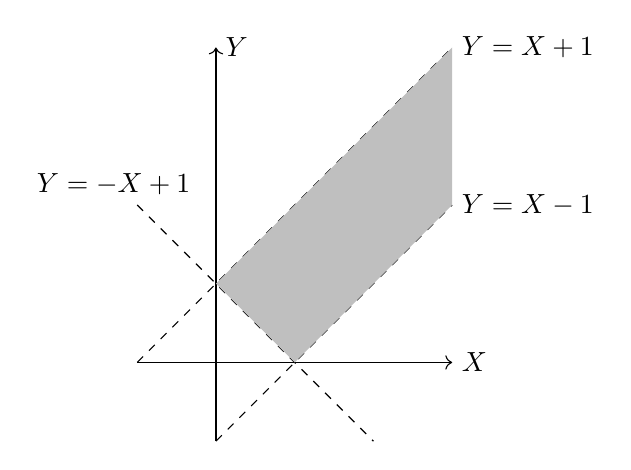
\begin{tikzpicture}[scale=1]
\draw [->] (-1, 0) -- (3, 0) node[right]{$X$}; 
\draw[->] (0, -1) -- (0, 4) node[right]{$Y$}; 
\draw[dashed, domain=-1:2] plot(\x, -\x+1);  
\draw (-1.3, 2) node[above]{$Y=-X+1$}; 
\draw[dashed, domain=0:3] plot(\x, \x-1) node[right]{$Y=X-1$}; 
\draw[dashed, domain=-1:3] plot(\x, \x+1) node[right]{$Y=X+1$}; 
\fill[lightgray] (1, 0)--(0, 1)--(3, 4)--(3, 2)--cycle;
\end{tikzpicture}
\end{center}
\caption{The image $\bP m(\Geo(C)/\bC)$ in $\bR\bP^2_{\geq 0}$.}
\end{figure}

\newpage

%============================================================
\section{The case of elliptic curves}\label{section-ell}
%\begin{itemize}
%    \item hom functions on the boundary (Koseki)
%    \item Compare with classical Teichmuller theory via mirror symmetry (Ouchi)
%    \item Relation with autoequivalences: 
%    Behaviour of fixed points vs positive entropy (Kikuta)
%\end{itemize}

%\subsection{Semistable objects on elliptic curves}
%\textcolor{red}{stable=spherical=indecomposable}
%subsectionに分けなくても良いかも



%\begin{prop}
%Let $X$ be an elliptic curve with a stability condition $\sigma \in \Stab(X)$.
%For a non-zero object $E \in D^b(X)$, the following are equivalent.
%\begin{itemize}
  %  \item[(1)] The object $E$ is $\sigma$-stable.
  %  \item[(2)] The object $E$ is spherical.
  %  \item[(3)] The object $E$ is indecomposable.
%\end{itemize}
%\begin{proof}
%\textcolor{red}{Cite}
%The statements $(1) \implies (2)$ and $(2) \implies (3)$ are evident.
%We prove the statement $(3) \implies (1)$. 
%Assume that the object $E$ is indecomposable. Shifting $E$, we may assume that $E$ is an indecomposable coherent sheaf on $X$.
%\end{proof}

%\end{prop}

The case of elliptic curves is discussed. 
We compare the Thurston compactification with the classical one of the torus via homological mirror symmetry in the first two subsections, 
and give the Nielsen--Thurston classification of autoequivalences in the rest. 

For an elliptic curve $X$, recall that we have 
\[
\Stab(X)=\Geo(X). 
\]
%in this case. 

\subsection{Homological mirror symmetry for elliptic curves}
In this subsection, we recall the homological mirror symmetry for elliptic curves following \cite{pz98}. 
For $\zeta\in \bH$, 
we consider the elliptic curve $X:=\bC/\bZ\oplus \zeta\bZ$ and a pair $\Tilde{X}:=(T_2,\zeta~dx \wedge dy)$, where $T_2=\bR^2/\bZ^2$ is the torus. Polishchuk and Zaslow \cite{pz98} constructed the equivalence 
\[\Phi_{\mathrm{PZ}}:D^b(X) \iso D^\pi\Fuk(\Tilde{X}).\]
Let $\pi: \bR^2 \to T_2$ be the natural projection.
Recall that an indecomposable object in the derived Fukaya category $D^\pi\Fuk(\Tilde{X})$ of $\Tilde{X}$ is isomorphic to a triple $(L, \lambda, M)$, where $L$ is a Lagrangian submanifold of $\Tilde{X}$ and $\lambda$ is a real number such that  
 \[L=\pi\left(\{ 
    z \in \bC \mid z=z_0+e^{i\pi\lambda}t, 
    ~ t \in \bR
    \}\right),\]
    and $M$ is a local system on $L$ whose monodoromy operators have only eigenvalues in the unitary group $U(1)$. 
    %For an object $(L,\lambda, M)$ in $D^\pi\Fuk(\Tilde{X})$, we have $(L,\lambda,M)[1]=(L,\lambda+1,M)$. 
    
    We define a surjective homomorphism 
    \[\cl:K(D^\pi\Fuk(\Tilde{X})) \to H_1(T_2,\bZ)\]
    as $\cl(L,\lambda,M):=[L]$ for $(L,\lambda,M) \in D^\pi\Fuk(\Tilde{X})$ with $\lambda \in (-1/2,1/2]$, 
    and extend it for a general element in 
    $D^\pi\Fuk(\tilde{X})$ 
    by using $(L,\lambda,M)[1]=(L,\lambda+1,M)$.
   For $(r_1,d_1),(r_2,d_2) \in H^{2*}(X,\bZ)$, we define the {\it Mukai pairing
 of $(r_1, d_1)$ and $(r_2,d_2)$} as 
 \[\langle(r_1,d_1), (r_2,d_2) \rangle:=r_1d_2-r_2d_1.\]
 For $E_1,E_2 \in D^b(X)$, we have 
\begin{equation}\label{eq:Riemann-Roch}
\chi(E_1,E_2)=\langle \ch(E_1), \ch(E_2)\rangle 
 \end{equation}
    by the Riemann--Roch formula. 
 From now on, we use the same notation as in Example \ref{ex:line segment}. 
We have an isomorphism 
    \[\varphi_{\mathrm{PZ}}:H^{2*}(X,\bZ) \iso H_1(T_2, \bZ), (r,d) \mapsto r \gamma_2+ d \gamma_1.\]
Note that $\varphi_{\mathrm{PZ}}$ is the isometry with respect to the Mukai pairing and the intersection pairing. Moreover, we have the following commutative diagram:

\begin{center}
\begin{tikzcd}
  K(X) \ar[r, "K(\Phi_{\mathrm{PZ}})"] \arrow[d, "\ch"'] & K(D^\pi\Fuk(\Tilde{X})) \ar[d, "\cl"'] \\
  H^{2*}(X,\bZ) \ar[r, "\varphi_{\mathrm{PZ}}"] & H_1(T_2,\bZ).
\end{tikzcd}
\end{center}

For an indecomposable coherent sheaf $E$ on $X$, the object $\Phi_{\mathrm{PZ}}(E)$ is isomorphic to a triple $(L,\lambda,M)$ such that
\[[L]=\rk (E) \gamma_2+ \deg (E) \gamma_1\] 
and $\lambda \in (-1/2,1/2]$. %by the above commutative diagram.  


Let $\mcP \in D^b(X\times X)$ be the normalized Poincar\'e line bundle of $X$. By \cite{muk81}, the Fourier-Mukai transform 
\[\Phi_\mcP: D^b(X) \to D^b(X),~ E \mapsto \mathbf{R}p_{1*}(p^*_2E \otimes \mcP)\]
is an autoequivalence, where $p_1$ and $p_2$ are the first projection and the second projection respectively. Then we have the cohomological Fourier-Mukai transform 
\begin{equation}\label{coh-Phi_P}
\Phi^H_\mcP:H^{2*}(X,\bZ) \iso H^{2*}(X,\bZ),~(r,d) \mapsto (d,-r), 
\end{equation}
which is an isometry with respect to the Mukai pairing.

We consider the equivalence 
\[\Tilde{\Phi}_{\mathrm{PZ}}:=\Phi_{\mathrm{PZ}} \circ \Phi^{-1}_{\mcP}:D^b(X) \iso D^\pi\Fuk(\Tilde{X})\]
and the isomorphism 
\[\Tilde{\varphi}_{\mathrm{PZ}}:=\varphi_{\mathrm{PZ}} \circ (\Phi^{-1}_{\mcP})^H: H^{2*}(X,\bZ) \iso H_1(T_2,\bZ).\]
For $(r,d) \in H^{2*}(X,\bZ),$ we have $\Tilde{\varphi}_{\mathrm{PZ}}(r,d)=-d\gamma_2+r\gamma_1$.

%For $E_1,E_2 \in D^b(X)$, we have 
%\[ \chi(E_1,E_2)=\rk(E_1)\deg(E_2)-\rk(E_2)\deg(E_1)\]
%by the Riemann-Roch formula. 
%Now, we can write
%\[cl\left(\Tilde{\Phi}_{\mathrm{PZ}}(E_1)\right)=\rk(E_1)\gamma_1-\deg(E_1)\gamma_2,\]
%\[cl\left(\Tilde{\Phi}_{\mathrm{PZ}}(E_2)\right)=\rk(E_1) \gamma_1-\deg(E_2)\gamma_2.\]
%Computing intersection numbers, we obtain
%\[\left(\rk(E_1)\gamma_1-\deg(E_1)\gamma_2 \right)\left(\rk(E_1) \gamma_1-\deg(E_2)\gamma_2 \right)=\langle\ch(E_1), \ch(E_2)  \rangle.\] 
\begin{rmk}\label{rmk:isometry}
The isomorphism $\Tilde{\varphi}_{\mathrm{PZ}}$ is isometry with respect to the Mukai pairing on $H^{2*}(X,\bZ)$ and the intersection pairing on $H_1(T_2,\bZ)$.
\end{rmk}


\begin{defin}\label{def:stability on Fukaya}
For a complex number $\beta+\sqrt{-1}\alpha \in \bH$, we define a stability condition $\Tilde{\sigma}_{\beta,\alpha}$ 
on $D^\pi\Fuk(\Tilde{X})$ with respect to $H_1(T_2, \bZ)$ 
as follows: 
\[\Tilde{\sigma}_{\beta,\alpha}:=(Z_{\beta, \alpha} \circ \Tilde{\varphi}^{-1}_{\mathrm{PZ}},\Tilde{\Phi}_{\mathrm{PZ}}(\Coh(X))).\]
\end{defin}


\begin{rmk}\label{rmk:period integral}
Central charges of the stability conditions in Definition \ref{def:stability on Fukaya} are related to period integrals.
Take a complex number $\tau=\beta+\sqrt{-1} \alpha \in \bH$. 
Then we have the orientation preserving diffeomorphism $f_\tau: T_2 \to  \bC/\bZ \oplus \tau\bZ$ in Example \ref{example:Teichmuler elliptic}. There is the unique holomorphic $1$-form $\Omega_\tau$ on the elliptic curve $\bC/\bZ \oplus \tau\bZ$ such that 
\[\int_{f_{\tau*}\gamma_1}\Omega_\tau=\tau, ~\int_{f_{\tau*}\gamma_2}\Omega_\tau=1. \]
Then we have the equality
\[\Tilde{Z}_{\beta, \alpha}(-)=\int_{(-)}\Tilde{\Omega}_\tau, \]
where $\Tilde{\Omega}_\tau:=f^*_\tau \Omega_\tau$.
In fact, we can prove this equality as follows.
First, note that the equality
\[\int_{\gamma_k}\Tilde{\Omega}_\tau=\int_{f_{\tau*}\gamma_k}\Omega_\tau\]
holds for $k=1,2$.
Take a class $\gamma=c_1 \gamma_1  + c_2 \gamma_2 \in H_1(T_2,\bZ)$, where $c_1$ and $c_2$ are integers. 
Then we obtain
\begin{align*}
    \Tilde{Z}_{\beta,\alpha}(\gamma) &= Z_{\beta, \alpha}(\Phi^H_\mcP \circ \varphi^{-1}_{\mathrm{PZ}}(\gamma)) \\
    &=Z_{\beta, \alpha}(c_1, -c_2)\\
    &=c_2+\tau c_1\\
    &=c_2 \int_{\gamma_2}\Tilde{\Omega}_\tau + c_1\int_{\gamma_1}\Tilde{\Omega}_\tau\\
    &= \int_{\gamma}\Tilde{\Omega}_\tau.
\end{align*}
\end{rmk}

%次のsubsectionに移動しても良いかも.





\subsection{Comparison of two Thurston compactifications}
In this subsection, we compare Thurston compactifications of spaces of stability conditions with Thurston compactifications of Teichm\"uller spaces in the case of elliptic curves.
We keep the notations as in the previous subsection. 

Recall that an object $E \in D^b(X)$ is called {\it spherical} if we have
\[ \mathbf{R}\Hom(E,E) \simeq \bC \oplus \bC[-1].\]


\begin{defin}
Let $\Sph(X)$ and $\Sph(\Tilde{X})$ be the sets of isomorphism classes of spherical objects in $D^b(X)$ and $D^\pi\Fuk(\Tilde{X})$ respectively.
\end{defin}

Spherical objects on elliptic curves are characterized as follows:

\begin{prop}\label{prop:spherical}
Let $\sigma \in \Stab(X)$ be a stability condition on $D^b(X)$.
Then a non-zero object $E \in D^b(X)$ is 
spherical if and only if it is $\sigma$-stable.
In particular, if $E$ is spherical, then we have $\gcd(\rk(E), \deg(E))=1$.
\end{prop}
\begin{proof}
Assume that $E$ is spherical. 
Since $\Hom(E,E)=\bC$, the object $E$ is indecomposable. By the proof of \cite[Theorem 8.1]{bri}, $E$ is a $\sigma$-semistable object. By \cite[Theorem 8.1]{bri} and taking shifts, we may assume that $E$ is a $\mu$-semistable sheaf on $X$. By \cite[Lemma 1, Proposition 4]{hp} and the equality $\Hom(E,E)=\bC$, $E$ is $\mu$-stable.
Therefore, $E$ is $\sigma$-stable.
The converse is easily deduced from the Serre duality.
\end{proof}
%Note that spherical objects on elliptic curves are semistable.
%\begin{rmk}
%By the proof of \cite[]{}, indecomposable objects in $D^b(X)$ are $\sigma$-semistable for any $\sigma \in \Stab(X)$. Since spherical objects are indecomposable, spherical objects in $D^b(X)$ are $\sigma$-semistable for any $\sigma \in \Stab(X)$.
%\end{rmk}

Now, we obtain the following proposition.
\begin{prop}\label{prop:mass=length}
Take a complex number $\tau \in \bH$ and put $t:=[f_\tau] \in \mcT(T_2)$. 
For a spherical object $(L, \lambda, M) \in D^\pi\Fuk(\Tilde{X})$, we have 
\[m_{\Tilde{\sigma}_{\beta,\alpha}}(L,\lambda,M)=l_{t}([L]). \]
\end{prop}
\begin{proof}
%There is integers $c_1, c_2$ such that $[L]=c_1\gamma_1+c_2\gamma_2$.
%As in the proof of {\cite[Theorem 8.1]{bri}}, the indecomposable  object $(L, \lambda, M)$ is %$\Tilde{\sigma}_{\beta,\alpha}$-semistable. 
By Proposition \ref{prop:spherical}, $(L, \lambda, M)$ is $\Tilde{\sigma}_{\beta,\alpha}$-stable.
Therefore, by example \ref{ex:line segment} and Remark \ref{rmk:period integral}, we obtain
\begin{align*}
m_{\Tilde{\sigma}_{\beta,\alpha}}(L,\lambda,M)&=\left|\Tilde{Z}_{\beta,\alpha}([L])\right|\\
&=\left| \int_{\gamma}\Tilde{\Omega}_\tau \right|\\
&=|c_2+\tau c_1|\\
&=l_t([L]).
\end{align*}
\end{proof}



Denote the space of stability conditions on $D^\pi\Fuk(\Tilde{X})$ with respect to $\cl$ by $\Stab(\Tilde{X})$.
The equivalence $\Tilde{\Phi}_{\mathrm{PZ}}:D^b(X) \iso D^\pi\Fuk(\Tilde{X})$ induces isomorphisms 
\[\Tilde{\Phi}_{\mathrm{PZ}}: \Stab(X)/\bC \iso \Stab(\Tilde{X})/\bC,\]
\[ \bP\left(\Tilde{\Phi}_{\mathrm{PZ}}\right): \bP^{\Sph(X)}_{\geq 0} \iso \bP^{\Sph(\Tilde{X})}_{\geq 0}, \]
\begin{rmk}\label{diag-mirror}
The above isomorphisms fit into the following commutative diagram: 
\begin{center}
\begin{tikzcd}
  \Stab(X)/\bC \ar[r, "\bP m"] \arrow[d, "\Tilde{\Phi}_{\mathrm{PZ}}"'] & \bP^{\Sph(X)}_{\geq 0} \ar[d, "\bP\Tilde{\Phi}_{\mathrm{PZ}}"'] \\
  \Stab(\Tilde{X})/\bC \ar[r, "\bP m"] & \bP^{\Sph(\Tilde{X})}_{\geq 0}.
\end{tikzcd}
\end{center}
\end{rmk}

Let $\mcS$ be the set of free homotopy classes of simple closed curves in $T_2$ as in Example \ref{ex:line segment}. 

\begin{comment}
\begin{rmk}\label{rmk:spherical class}
Take $\gamma=c_1\gamma_1+c_2\gamma_2 \in \mcS$. Since $\gcd(c_1,c_2)=1$, there exist an integer $n$ and a $\mu$-stable sheaf $E$ on $X$ with $\ch(E[n])=(c_1,c_2)$.
By Proposition \ref{prop:spherical}, $E[n]$ is a spherical object in $D^b(X)$.
Then the object $\Phi_{\mathrm{PZ}}(E)$ is isomorphic to an object of the form $(L,\lambda,M)$ such that $[L]=c_1\gamma_1+c_2\gamma_2$. 
\textcolor{red}{This seems to explain an association $\mcS \to \Sph(\tilde{X})$, but we need a map $\Sph(\tilde{X}) \to \mcS$ for Def. 5.8? 
Seems to be enough to explain that 
$[L] \in \mcS$ for all $(L, \lambda, M) \in \Sph(\tilde{X})$?
And, we use this fact in the statement  of Thm 5.10 (2). }
\end{rmk}
\end{comment}


\begin{rmk}\label{rmk:spherical class}
For $(L,\lambda, M) \in \Sph(\tilde{X})$, 
there are integers $c_1$ and $c_2$ such that $[L]=c_1 \gamma_1+c_2 \gamma_2$ and $\gcd(c_1,c_2)=1$ by the equivalence $\Tilde{\Phi}_{\mathrm{PZ}}$ and Proposition \ref{prop:spherical}.
\end{rmk}

By Proposition \ref{prop:spherical} and Remark \ref{rmk:spherical class}, 
we can define the following map.

\begin{defin}
Take a point $x=(x_{\gamma})_{\gamma \in \mcS} \in \bP^{\mcS}_{\geq 0}$. 
For a spherical object $(L,\lambda,M) \in \Sph(\Tilde{X})$, we define 
$y_{(L,\lambda,M)}:=x_{[L]}$. Defining
\[\iota(x):=(y_{(L,\lambda,M)})_{(L,\lambda,M)\in \Sph(\Tilde{X})}, \]
we obtain an injective continuous map
\[\iota:\bP^{\mcS}_{\geq 0} \to \bP^{\Sph(\Tilde{X})}_{\geq 0}. \]
\end{defin}

By the isomorphism (\ref{isomorphism:H vs Stab}), we have the isomorphism 
\[\varepsilon : \bH \iso \Stab(X)/\bC. \]
We consider the isomorphism 
\[\eta:=\Tilde{\Phi}_{\mathrm{PZ}} \circ \varepsilon \circ \xi^{-1}: \mcT(T_2) \iso \Stab(\Tilde{X})/\bC,\]
where $\xi:\bH \iso \mcT(T_2)$ is the isomorphism in Example \ref{example:Teichmuler elliptic}. For $\tau=\beta+\sqrt{-1}\alpha \in \bH$, we have $\eta([f_\tau])=\Tilde{\sigma}_{\beta,\alpha}$. 

\begin{defin}\label{def-intersection}
We define functions $i_X$ and $i_{\Tilde{X}}$ as follows: 
\[i_X:\Sph(X)\times\Sph(X) \to \bZ_{\geq 0}, \quad 
(E,F) \mapsto |\chi(E,F)|,\]
\[i_{\Tilde{X}}:\Sph(\Tilde{X})\times\Sph(\Tilde{X}) \to \bZ_{\geq 0}, \quad 
(E,F) \mapsto |\chi(E,F)|.\]
Then we define maps $i_{X*}$ and $i_{\Tilde{X}*}$ 
as in Question \ref{ques:Thurston compactification} (3): 
%As in Theorem \ref{thm:Thurston comactification}, we define the functions
 %\[i_{X*}(E):\Sph(X) \to \bZ_{\geq 0},\]
 %\[i_{\Tilde{X}*}(E):\Sph(\Tilde{X}) \to \bZ_{\geq 0}\]
 %for a spherical object $E$ in $D^b(X)$ and $D^\pi\Fuk(\Tilde{X})$ respectively. 
\begin{equation*}
i_{X*}:\Sph(X) \to \bP^{\Sph(X)}_{\geq 0}, \quad
i_{\Tilde{X}*}:\Sph(\Tilde{X}) \to \bP^{\Sph(\Tilde{X})}_{\geq 0}. 
\end{equation*}
\end{defin}

Recall that
\begin{eqnarray*}
\overline{\Stab(X)/\bC}&:=&\overline{\bP m(\Stab(X)/\bC)}\\
\partial\Stab(X)/\bC&:=&\left(\overline{\Stab(X)/\bC}\right)\backslash\bP m\left(\Stab(X)/\bC\right), 
\end{eqnarray*}
cf. Question \ref{ques:Thurston compactification} (2),(3). 
The following is the main theorem of this section. 
\begin{thm}\label{thm:main elliptic}
The following diagram commutes:
\begin{center}
\begin{tikzcd}
  \Stab(X)/\bC \ar[r, hookrightarrow, "\bP m"] \arrow[d, "\sim"sloped, "\Tilde{\Phi}_{\mathrm{PZ}}"'] & \bP^{\Sph(X)}_{\geq 0} \ar[d, "\sim"sloped, "\bP\Tilde{\Phi}_{\mathrm{PZ}}"'] \\
  \Stab(\Tilde{X})/\bC \ar[r, hookrightarrow, "\bP m"] & \bP^{\Sph(\Tilde{X})}_{\geq 0}\\
      \mcT(T_2) \ar[r, hookrightarrow, "\bP l "] \arrow[u, "\eta", "\sim"'sloped] & \bP^{\mcS}_{\geq 0} \arrow[u, "\iota", hookrightarrow].
\end{tikzcd}
\end{center}
Furthermore, the following statements hold.
\begin{itemize}
    \item[(1)] The maps given by the restrictions
    \[\bP \Tilde{\Phi}_{\mathrm{PZ}}: \overline{\Stab(X)/\bC} \to \overline{\Stab(\Tilde{X})/\bC},
\]
\[\iota:\overline{\mcT(T_2)} \to \overline{\Stab(\Tilde{X})/\bC}, 
\]
are homeomorphisms.
\item[(2)]%Let $i(-.-):\mcS \times \mcS \to \bZ_{\geq 0}$ be the function in Theorem \ref{thm:Thurston comactification}. 
For $E \in \Sph(X)$ with $\Tilde{\Phi}_{\mathrm{PZ}}(E)=(L,\lambda,M)$, we have 
\[\bP\Tilde{\Phi}_{\mathrm{PZ}} (i_{X*}(E))=i_{\Tilde{X}*}(L,\lambda,M)=\iota(i_{*}(\cl(L,\lambda,M))). \]



In particular, we obtain 
\[\partial \Stab(X)/\bC=\overline{i_{X*}(\Sph(X))},\]
\[\partial \Stab(\Tilde{X})/\bC=\overline{i_{\Tilde{X}*}(\Sph(\Tilde{X}))}.\]

\end{itemize}
\end{thm}
\begin{proof}
The commutativity of the diagrams is deduced from Remark \ref{diag-mirror} and Proposition \ref{prop:mass=length}. 
%\textcolor{red}{for which square are you using Prop 5.6?}

We prove the statement (1).
Since $\iota$ is continuous, we have $\iota\left(\overline{\mcT(T_2)}\right) \subset \overline{\iota(\bP l(\mcT(T_2)))}=\overline{\Stab(\Tilde{X})/\bC}$. Therefore, we obtain the injective continuous map 
$\iota: \overline{\mcT(T_2)} \to \overline{\Stab(\Tilde{X})/\bC}$.
Since $\overline{\mcT(T_2)}$ is compact and $\overline{\Stab(\Tilde{X})/\bC}$ is Hausdorff, $\iota: \overline{\mcT(T_2)} \to \overline{\Stab(\Tilde{X})/\bC}$ is a homeomorphism onto its image. Since $\iota\left(\overline{\mcT(T_2)}\right)$ is a compact subspace of the Hausdorff space  $\overline{\Stab(\Tilde{X})/\bC}$, $\iota\left(\overline{\mcT(T_2)}\right)$ is closed. 
By the inclusion $\bP m(\Stab(\Tilde{X})/\bC) \subset \iota\left(\overline{\mcT(T_2)}\right)$, we obtain \[  \iota\left(\overline{\mcT(T_2)}\right)=\overline{\Stab(\Tilde{X})/\bC}.\]

Next, we prove the statement (2). 
Take $(L',\lambda',M') \in \Sph(\Tilde{X})$. Then we have 
\begin{align*}
    \bP \Tilde{\Phi}_{\mathrm{PZ}}(i_{X*}(E))(L',\lambda',M')&=i_{X*}(E)(\Tilde{\Phi}^{-1}_{\mathrm{PZ}}(L',\lambda',M')) \\
    &=i_{X}(E,\Tilde{\Phi}^{-1}_{\mathrm{PZ}}(L',\lambda',M'))\\
    &=i_{\Tilde{X}}((L,\lambda,M),(L',\lambda',M'))\\
    &=i_{\Tilde{X}*}(L, \lambda, M)(L',\lambda',M')
\end{align*}
by (\ref{eq:Riemann-Roch}) and Remark \ref{rmk:isometry}. and 
\begin{align*}
    \iota(i_{*}(\cl(L,\lambda,M)))(L',\lambda',M')&=i([L],[L'])\\
    &=i_{\Tilde{X}*}(L,\lambda,M)(L',\lambda',M')
\end{align*}
by Example \ref{ex:line segment}.
%\textcolor{red}{(5.1) and Rmk 5.1 are used for the former equations, while Ex 3.3 is for the latter. 
%Maybe better to make it clearer which is used for which?}
\end{proof}

%\textcolor{red}{refer to Theorem 3.4}

By Theorem \ref{thm:main elliptic}, we obtain an affirmative answer to Question \ref{ques:Thurston compactification} (3) for an elliptic curve $X$.

%============================================================
\begin{comment}
\subsection{Description of boundaries}
The following lemma shows that 
the above choice (\ref{eq:Ssph}) of the set $\mcS$ is natural: 

\textcolor{red}{spherical=simple=stable (use FM transform)}
\begin{lem}
Let $C$ be an elliptic curve. 
The following statements hold: 
\begin{enumerate}
    \item An object $E \in D^b(C)$ is spherical 
    if and only if it is a shift of a simple sheaf. 
    \item A simple sheaf $E \in \Coh(C)$ is slope semistable. 
\end{enumerate}
\end{lem}
\begin{proof}
(1) A shift of a simple sheaf is obviously spherical. 
On the other hand, let $E \in D^b(C)$ be a spherical object. 
Then it decomposes as 
\[
E \cong \bigoplus_i \mcH^i(E)[-i]. 
\]
Since we assume the object $E$ is spherical, 
we in particular have $\hom(E, E)=1$. 
Hence it must be concentrated in one cohomological degree, 
i.e., we have $E=F[n]$ for some coherent sheaf $F$ 
and integer $n \in \bZ$. 
Since we have the equation $\hom(F, F)=\hom(E, E)=1$, 
we conclude that $F$ is simple. 

(2) Suppose that $E$ is unstable. 
Then there exists a non-zero sheaves 
$A, B \in \Coh(C)$ with 
$\mu_{\min}(A) > \mu_{\max}(B)$ 
and an exact sequence 
\[
0 \to A \to E \to B \to 0. 
\]
On the other hand, by Serre duality we have 
\[
\Ext^1(B, A) \cong \Hom(A, B)^\vee=0, 
\]
where the second equality follows from 
the inequality $\mu_{\min}(A) > \mu_{\max}(B)$. 
We conclude that $E \cong A \oplus B$, 
and hence $E$ is not simple. 
\end{proof}

%============================================================

\begin{defin}
For an object $a \in \mcS$, 
we define a function 
$\overline{\hom}(a) \colon \mcS \to \bR$ by 
\[
\overline{\hom}(a)(x):=
\begin{cases}
0 & (x \mbox{ is a shift of } a) \\
\sum_i \ext^i(a, x) & (otherwise). 
\end{cases}
\]

We also denote by 
$\overline{\hom}(a) \in \bP^\mcS$ 
its projection via 
$\bR^{\mcS} \setminus \{0\} \to \bP^\mcS$. 
(\textcolor{blue}{Check the well-definedness at least for elliptic curves, i.e., check 
$\overline{\hom}(a) \neq 0 \in \bR^\mcS$
This should be true according to the following Prop.}. 
)
\end{defin}

\begin{rmk}
$\overline{\hom}(a)(x)=|\chi(a, x)|$. 
\end{rmk}


\textcolor{red}{Is this a correct definition? 
\cite{bdl20} seems to use this definition, although 
they does NOT give a precise definition!!!}

\begin{prop}
Let $C$ be an elliptic curve, 
take spherical objects $a, x \in \mcS$ 
and a stability conditions $\sigma \in \Stab(C)$. 
Then we have 
\[
\lim_{n \to \infty}\frac{m_{\sigma}(\ST^n_a(x))}{n}
=m_\sigma(a) \cdot \overline{\hom}(a)(x). 
\]
\end{prop}
\begin{proof}
Idea: 
\begin{enumerate}
    \item By shifting $a \in \mcS$ if necessary, 
    we may assume $a$ is a sheaf. 
    Put $v:=\ch(a)$. 
    Then the moduli space $M_v$ of simple sheaves 
    with Chern character $v$ is isomorphic to $C$. (???)
    
    \item Using Fourier--Mukai $D^b(C) \cong D^b(M_v)$ 
    induced by the universal family, 
    reduce the problem to the case of 
    $a=\mcO_p$ for some $p \in C$. 
    
    \item 
    Up to $\bC$-action, 
    we may assume $\sigma=\sigma_{\beta, \alpha}$. 
    When $a=\mcO_p$, we have 
    $\ST_a=(-) \otimes \mcO_C(p)$. 
    Since $\ch(x \otimes \mcO(np))
    =(\rk(x), \deg(x)+n\rk(x))$, 
    the left hand side is 
    $\rk(x)$. 
    
    For the right hand side, 
    $m_{\sigma_{\beta, \alpha}}(\mcO_p)=1$, 
    and 
    \[
    \overline{\hom}(\mcO_p)(x)=
    \begin{cases}
    0=\rk(x) & (x=\mcO_q[k], q \in C, k \in \bZ) \\
    \rk(x) & (x \mbox{ is a shift of a vector bundle, by RR}). 
    \end{cases} \\
    \]
\end{enumerate}

\end{proof}

\begin{prop}
The set of $\overline{\hom}(a)$ are dense in Thurston boundary. 
\end{prop}
\begin{proof}

\end{proof}

%============================================================
\subsection{Elliptic curves and Fourier--Mukai transforms}
%後で形式を整える.
In this subsection, we recall the properties of Fourier--Mukai transforms for elliptic curves.

Let $X$ be an elliptic curve. 
For coprime integers $r,d \in \bZ$ satisfying $r>0$, let $M(r,d)$ be the moduli space of $\mu$-semistable sheaves with Chern character $(r,d)$. Then the moduli space $M(r,d)$ has an universal family $\mcU_{r,d}$ and it induces the Fourier--Mukai transform $\Phi_{\mcU_{r,d}}\colon D^b(M(r,d))\xrightarrow{\sim}D^b(X)$. 
\end{comment}

%============================================================
\subsection{Nielsen--Thurston classification of autoequivalences and the categorical entropy}
%Relation with autoequivalences: Behaviour of fixed points vs positive (categorical, topological) entropy
Here, we consider an analogue of the classical Nielsen--Thurston classification of the torus
for autoequivalences of elliptic curves, and its relation to the categorical entropy. 

%------------------------------------------------------------
\subsubsection{${\rm PSL}(2,\bZ)$-actions}
\begin{comment}
Note that an object $E \in D^b(X)$ is a spherical object if and only if we have the equality $\Hom(E,E)=\bC$. For a spherical object $E \in D^b(X)$, denote the spherical twist around $E$ by $T_{E}$. For an object $A \in D^b(X)$, there is the exact triangle
\[\RHom(E,A)\otimes E \to A \to T_E(A), \]
where the first morphism is the evaluation map.
\end{comment}

%N(D^b(x))のbasisの固定
%Poincare bdlに関するFM変換
%生成元の対応
Taking the cohomological Fourier--Mukai transforms, 
we have an exact sequence
\begin{equation}\label{ell-ex}
1 \to \left(\Aut(X) \ltimes \Pic^0(X) \right) \times \bZ[2] \to \Aut(D^b(X)) \to \SL(2,\bZ) \to 1.
\end{equation}

%============================================================


The exact sequence (\ref{ell-ex}) induces an isomorphism 
\[
\rho:~\Gamma(X):=\Aut(D^b(X))/\left((\Aut(X) \ltimes \Pic^0(X))\times \bZ[1]\right)
\xrightarrow{\sim}
{\rm  PSL}(2,\bZ)
.
\]
%-----
\begin{comment}
For our purpose, we fix the modified version as follows
\[
\rho_1:~\Gamma(X)\xrightarrow{\sim}{\rm  PSL}(2,\bZ);~\Phi\mapsto
\begin{pmatrix}
0 & 1 \\
1 & 0 \\
\end{pmatrix}
\rho(\Phi)
\begin{pmatrix}
0 & 1 \\
1 & 0 \\
\end{pmatrix}
.
\]
Since the group $\left(\Aut(C) \ltimes \Pic^0(C) \right) \times \bZ[1]$ acts on $\Stab(C)/\bC$ trivially, 
we can define the action of ${\rm PSL}(2,\bZ)$ on $\Stab(C)/\bC$ via this isomorphism $\rho_1$,   
and notice that ${\rm PSL}(2,\bZ)$ naturally acts on $\bH$ by M\"{o}bius transformations. 

\begin{prop}
For the above actions of ${\rm PSL}(2,\bZ)$,  
the isomorphism 
\[
\varphi:\bH \xrightarrow{\sim} \Stab(C)/\bC
\]
is ${\rm PSL}(2,\bZ)$-equivariant. 
\end{prop}
\begin{proof}
It suffices to check that generators $\Phi_P,~-\otimes\mcO_C(p)$ of $\Gamma(X)$ satisfy the equivariant condition. 
Note that 
\[
\rho_1(\Phi_P)
=
\begin{pmatrix}
0 & -1 \\
1 & 0 \\
\end{pmatrix}
\text{ and }
\rho_1(-\otimes\mcO_C(p))
=
\begin{pmatrix}
1 & 1 \\
0 & 1 \\
\end{pmatrix}
.
\]
For each $\beta+\sqrt{-1}\alpha\in\bH$, we have

, hence
\[
\varphi
\left(
\begin{pmatrix}
0 & -1 \\
1 & 0 \\
\end{pmatrix}
.(\beta+\sqrt{-1}\alpha)
\right)
=
\begin{pmatrix}
0 & -1 \\
1 & 0 \\
\end{pmatrix}
.
\varphi(\beta+\sqrt{-1}\alpha)
\]
Similarly, we can check that
\[
\varphi
\left(
\begin{pmatrix}
1 & 1 \\
0 & 1 \\
\end{pmatrix}
.(\beta+\sqrt{-1}\alpha)
\right)
=
\begin{pmatrix}
1 & 1 \\
0 & 1 \\
\end{pmatrix}
.
\varphi(\beta+\sqrt{-1}\alpha)
, 
\]
which completes a proof. 
\end{proof}
\end{comment}
%-----
Since the group $\mcI(X):=\left(\Aut(X) \ltimes \Pic^0(X) \right) \times \bZ[1]$ acts on $\Stab(X)/\bC$ trivially, 
$\Gamma(X)$ naturally acts by isometries on $\Stab(X)/\bC$ with respect to the quotient metric $\bar{d}_B$ of $d_B$ by the $\bC$-action. 

We consider an action of ${\rm  PSL}(2,\bZ)$ on $\bH$
as a variant of M\"{o}bius transformation given by 
\begin{equation}\label{var-Mobius}
A.z:=
\left(
\begin{pmatrix}
0 & 1 \\
1 & 0 \\
\end{pmatrix}
A
\begin{pmatrix}
0 & 1 \\
1 & 0 \\
\end{pmatrix}
\right)
._Mz
\end{equation}
for $A\in{\rm  PSL}(2,\bZ)$ and $z\in\bH$, 
where the action $._M$ on the right hand side is the usual M\"{o}bius transformation
%Since the matrix is an involution, this action is well-defined. 
\[
\begin{pmatrix}
a & b \\
c & d \\
\end{pmatrix}
._Mz:=
\frac{az+b}{cz+d}
.
\]
\begin{rmk}\label{rem-var-Mobius}
\begin{enumerate}
\item
Clearly, the action (\ref{var-Mobius}) 
of ${\rm  PSL}(2,\bZ)$ is also isometric with respect to the hyperbolic metric $d_H$ on $\bH$. 
\item
Since the trace is invariant under taking the conjugation, 
for (a representative of) $A\in{\rm  PSL}(2,\bZ)$, we have 
\[
|{\rm tr}A|
=
\left |{\rm tr}
\begin{pmatrix}
0 & 1 \\
1 & 0 \\
\end{pmatrix}
A
\begin{pmatrix}
0 & 1 \\
1 & 0 \\
\end{pmatrix}
\right |.
\]

\end{enumerate}
\end{rmk}
%We use the action (\ref{var-Mobius}) below. 
\begin{prop}\label{psl-equiv}
Via the identification $\rho^{-1}:{\rm  PSL}(2,\bZ)\xrightarrow{\sim}\Gamma(X)$,   
the homeomorphism
\[
\varphi:(\bH, d_H) \xrightarrow{\sim} (\Stab(C)/\bC, \bar{d}_B)
\]
is ${\rm PSL}(2,\bZ)$-equivariant and isometric (up to a multiplicative constant). 
\end{prop}
\begin{proof}
By the formula (\ref{coh-Phi_P}), we have 
\[
\rho(\Phi_\mcP)
=
\begin{pmatrix}
0 & 1 \\
-1 & 0 \\
\end{pmatrix}
\text{ and }
\rho(-\otimes\mcO_C(p))
=
\begin{pmatrix}
1 & 0 \\
1 & 1 \\
\end{pmatrix}
.
\]
Hence $\Phi_\mcP$ and $-\otimes\mcO_C(p)$ generate $\Gamma(X)(\simeq{\rm  PSL}(2,\bZ))$. 
It suffices to check that these generators satisfy the equivariance condition. 

For each $\beta+\sqrt{-1}\alpha\in\bH$, we set 
\[
\tau:=
\varphi
\left(
\begin{pmatrix}
0 & 1 \\
-1 & 0 \\
\end{pmatrix}
.(\beta+\sqrt{-1}\alpha)
\right)
\in\Stab(X)/\bC. 
\]
Then direct computations show that 
\begin{eqnarray*}
Z_\tau&=&Z_{\frac{-1}{\beta+\sqrt{-1}\alpha}}\\
&=&\frac{1}{\beta+\sqrt{-1}\alpha}Z_{\beta+\sqrt{-1}\alpha}\circ\Phi_\mcP^{-1}\\
&=&\frac{1}{\beta+\sqrt{-1}\alpha}Z_{(\Phi_\mcP.\sigma_{\beta+\sqrt{-1}\alpha})}. 
\end{eqnarray*}
By Lemma \ref{curv-stab-determined-by-central}, we have 
\[
\varphi
\left(
\begin{pmatrix}
0 & 1 \\
-1 & 0 \\
\end{pmatrix}
.(\beta+\sqrt{-1}\alpha)
\right)
=
\begin{pmatrix}
0 & 1 \\
-1 & 0 \\
\end{pmatrix}
.
\varphi(\beta+\sqrt{-1}\alpha).
\]
Similarly, we can check that
\[
\varphi
\left(
\begin{pmatrix}
1 & 0 \\
1 & 1 \\
\end{pmatrix}
.(\beta+\sqrt{-1}\alpha)
\right)
=
\begin{pmatrix}
1 & 0 \\
1 & 1 \\
\end{pmatrix}
.
\varphi(\beta+\sqrt{-1}\alpha). 
\]
Thus $\varphi$ is ${\rm PSL}(2,\bZ)$-equivariant. 

Let 
\[
\varphi_-:(\bH, d_H) \xrightarrow{\sim} (\bH, d_H);~\beta+\sqrt{-1}\alpha\mapsto -\beta+\sqrt{-1}\alpha
\]
be an orientation reversing isometry, and 
\[
\varphi_W:(\bH, d_H) \xrightarrow{\sim} (\Stab(C)/\bC, \bar{d}_B);~\beta+\sqrt{-1}\alpha\mapsto
\overline{\sigma_{0,1}.
\widetilde{
\begin{pmatrix}
\alpha & \beta \\
0 & 1 \\
\end{pmatrix}
}
}
\]
an identification, 
where
$\widetilde{
\begin{pmatrix}
\alpha & \beta \\
0 & 1 \\
\end{pmatrix}
}$
is a lift of the matrix 
$
\begin{pmatrix}
\alpha & \beta \\
0 & 1 \\
\end{pmatrix}
$
via the universal covering
$
\widetilde{{\rm GL}}_+(2,\bR)\to{\rm GL}_+(2,\bR).
$
Using Lemma \ref{curv-stab-determined-by-central}, 
it is easy to check that 
\[
\overline{\sigma_{0,1}.
\widetilde{
\begin{pmatrix}
\alpha & \beta \\
0 & 1 \\
\end{pmatrix}
}
}
=\overline{\sigma_{-\beta,\alpha}}. 
\]
By Woolf's computation (\cite[Proposition 4.1]{Woo}), $\varphi_W$ is isometric (up to 
scaling by $1/2$). 
%(multiplied by $\frac{1}{2}$) 
Therefore the map $\varphi=\varphi_W\circ\varphi_-$ is also isometric, which completes the proof. 
\end{proof}
Since ${\rm  PSL}(2,\bZ)$ is isomorphic to the isometry group of $(\bH, d_H)$, the following is a direct corollary of the above proposition. 
\begin{cor}\label{non-trivial}
Let $\Phi$ be an autoequivalence of $D^b(X)$. 
Then, $\Phi$ is non-trivial in $\Gamma(X)$ if and only if 
$\Phi$ acts on $\Stab(X)/\bC$ non-trivially. 
\end{cor}
\begin{comment}
Set
\[
\overline{\Stab(X)/\bC}:=\overline{{\bP m}(\Stab(X)/\bC)}
\]
and
\[
\partial(\Stab(X)/\bC)
:=(\overline{\Stab(X)/\bC})\backslash {\bP m}(\Stab(X)/\bC). 
\]
\end{comment}
By Lemma \ref{lem:defbarm} and the proof of Theorem \ref{thm:closure}, 
we can extend the isometry $\varphi$ 
to the isomorphism 
$\overline{\bH} \xrightarrow{\sim} \overline{\Stab(X)/\bC}$. 
%\[
%m\circ\varphi:~\overline{\bH}\xrightarrow{\sim} \overline{m(\Stab(C)/\bC)}\subset
%\]
Also, the action of $\Gamma(X)$ can be extended to its action by homeomorphisms on the compactification $\overline{\Stab(X)/\bC}$ by Proposition \ref{psl-equiv}. 
%In general, quasi-isometry can be extended to a homeo cf. [FM, Thm 8.7]. 

%------------------------------------------------------------
\subsubsection{Nielsen--Thurston classification}
The {\it translation length} $l_B(\Phi)\in\bR_{\ge0}$ of $\Phi\in\Aut(D^b(X))$
with respect to the isometric action on $(\Stab(X)/\bC,\bar{d}_B)$ is given by
\[
l_B(\Phi):=\displaystyle\inf_{\sigma\in \Stab(X)/\bC}\bar{d}_B(\sigma,\Phi.\sigma). 
\]
\begin{defin}
%[{\cite[Ch II.6 Definition 6.3]{BriH}}]
Let $\Phi\in\Aut(D^b(X))$ be an autoequivalence. 
\begin{enumerate}
\item
$\Phi$ is {\it elliptic} if 
there exists $\sigma\in\Stab(X)/\bC$ such that $l_B(\Phi)=\bar{d}_B(\sigma,\Phi.\sigma)$ and $l_B(\Phi)=0$, or equivalently $\Phi$ has a fixed point in $\Stab(X)/\bC$. 
\item
$\Phi$ is {\it parabolic} if $l_B(\Phi)$ does not attain its minimum. 
\item
$\Phi$ is {\it hyperbolic} if 
there exists $\sigma\in\Stab(X)/\bC$ such that $l_B(\Phi)=\bar{d}_B(\sigma,\Phi.\sigma)$ and $l_B(g)>0$.
\end{enumerate}
\end{defin}
\begin{comment}
Note that 
\[
{\rm tr}
\begin{pmatrix}
0 & 1 \\
1 & 0 \\
\end{pmatrix}
A
\begin{pmatrix}
0 & 1 \\
1 & 0 \\
\end{pmatrix}
=
{\rm tr }A
\]
for $A\in{\rm SL}(2,\bZ)$, 
thus the trichotomy: elliptic, parabolic and hyperbolic, is preserved. 
\end{comment}
We give the characterizations of the above trichotomy of isometries. 
%elliptic
\begin{prop}\label{prop-ell}
Let $\Phi\in\Aut(D^b(X))$ be an autoequivalence which is non-trivial in $\Gamma(X)$. 
The following conditions are equivalent. 
\begin{enumerate}
\item
$\Phi$ is elliptic. 
\item
$|{\rm tr}\rho(\Phi)|<2$. 
\item
$\Phi$ has a unique fixed point in $\Stab(X)/\bC$. 
\item
(periodic) There exists a positive integer $m\in\bZ_{>0}$ such that $\Phi^m\in\mcI(X)$. 
%\mcI(X)や\Pic^0の元は(up to shiftで)有限位数になり得る?
\end{enumerate}
\end{prop}
\begin{proof}
%Since the trace is invariant under taking the conjugation by the matrix $\begin{pmatrix}
%0 & 1 \\
%1 & 0 \\
%\end{pmatrix}$, 
By Remark \ref {rem-var-Mobius} (2) and Proposition \ref{psl-equiv}, 
the conditions (1), (2) and (3) are all equivalent by the classical facts on M\"{o}bius transformation, see \cite[Section 13.1]{FM}. 

These three conditions are also equivalent to the finiteness of the order of $\Phi$ in $\Gamma(X)$(\cite[Section 13.1]{FM}), i.e., to the condition (4). 
\end{proof}

%parabolic
\begin{prop}\label{prop-para}
Let $\Phi\in\Aut(D^b(X))$ be an autoequivalence which is non-trivial in $\Gamma(X)$. 
The following conditions are equivalent. 
\begin{enumerate}
\item
$\Phi$ is parabolic. 
\item
$|{\rm tr}\rho(\Phi)|=2$. 
\item
$\Phi$ has a unique fixed point in $\partial(\Stab(X)/\bC)$. 
\item
(reducible) There exists a spherical object $E\in D^b(X)$ and $\Psi\in\mcI(X)$ such that $\Phi(E)=\Psi(E)$. 
%\mcI(X)や\Pic^0の元は(up to shiftで)任意のspherical objを固定する?数値類に推移的に作用する?
%primitive rational vectorはspherical class?
%transitive action of $\mcI(X)$ on a fixed spherical class

\begin{comment}
\item
(reducible)
There exists a spherical object $E\in D^b(X)$ such that 
\[
\ch(\Phi E)=\ch(E) \ \text{or} \ \ch(\Phi E)=-\ch(E). 
\]
%\mcI(X)や\Pic^0の元は(up to shiftで)任意のspherical objを固定する?数値類に推移的に作用する?
%導来同値と平行移動でtransitiveを示す
%primitive rational vectorはspherical class objで代表される(ch=rk/degな安定ベクトル束)

\item
%$\mcN(\Phi)$ fixes a $2-$class up to sign. 
There uniquely exists a $2$-class $v \in H^{2*}(X,\bZ)$
%$v\in\mcN(D^b(X))$ 
such that 
\[\Phi^H(v)=v \ \text{or} \ \Phi^H(v)=-v. \]
%\[
%\mcN(\Phi)v=v \text{ or }\mcN(\Phi)v=-v. 
%\]
\end{comment}

\end{enumerate}
\end{prop}
\begin{proof}
%Since the trace is invariant under taking conjugations, 
By Remark \ref {rem-var-Mobius} (2) and Proposition \ref{psl-equiv}, 
the conditions (1),(2) and (3) are all equivalent by the classical facts on M\"{o}bius transformation, see \cite[Section 13.1]{FM}. 

We prove $(3)\Rightarrow(4)$. 
%Via the surjection $\Aut(D^b(X))\twoheadrightarrow{\rm  SL}(2,\bZ)$,
The cohomological Fourier--Mukai transform $\Phi^H \in \SL(2, \bZ)$ fixes (up to sign) a primitive integral vector $v\in\bR^2$ %as an eigenvector 
(\cite[Section 13.1]{FM}), 
which is also a cohomology class of a spherical object. 
By Proposition \ref{prop:spherical}, we can take a $\mu$-stable sheaf $E$ satisfying $\ch(E)=v$. 
By composing with shifts if necessary, we may assume that $\Phi (E)$ is also a $\mu$-stable sheaf. 
Then since $\rk E>0$ and $\rk\Phi(E)>0$, 
we have $\ch(\Phi (E))=\ch(E)$. 
\begin{comment}
(equivalently, taking shifts, a $\mu$-stable sheaf by Proposition \ref{prop:spherical}) $E\in D^b(X)$: 
\[
\ch(\Phi (E))=\ch(E) \ \text{or} \ \ch(\Phi (E))=-\ch(E). 
\]
By composing with a shift if necessary, we may assume that $\ch(\Phi (E))=\ch(E)$.     
\end{comment}
Set $\ch(E)=(r,d)$.
%with $r>0$. 
It is well-known that there exists an autoequivalence $F_{r,d}\in\Aut(D^b(X))$, 
which yields a one-to-one correspondence between the structure sheaf $\mcO_x$ of a point $x\in X$ and a $\mu$-stable sheaf $F_{r,d}(\mcO_x)$ of rank $r$ and degree $d$ (\cite[Proposition 3]{hp}). 
%such that 
%for each point $p\in X$, $F_{r,d}(\mcO_p)$ is a $\mu$-stable sheaf of rank $r$ and degree $d$ (\cite{}). 
%Conversely, for any $\mu$-stable sheaf $E'$ of rank $r$ and degree $d$, $F_{r,d}^{-1}(E')$ is a structure sheaf of a point. 
Let $f\in\Aut(X)$ be a translation satisfying 
\[
f^*(F_{r,d}^{-1}(E))=F_{r,d}^{-1}\Phi (E). 
\]
Since $f^*$ (composed with shifts) is an element of $\mcI(X)$, so is the conjugation $F_{r,d}\circ f^*\circ F_{r,d}^{-1}$. 
This autoequivalence is our desired $\Psi$. 
%Via the identifications  $H^{2*}(X,\bZ)\simeq\bZ\oplus\bZ$ and $\rho:\Gamma(X)\simeq{\rm  PSL}(2,\bZ)$, 
%the claim (4) is equivalent to the above three claims, \cite{FM}. 

The assertion $(4)\Rightarrow(2)$ easily holds by the following argument. 
The condition (4) implies that 
$\Phi^H \in \SL(2, \bZ)$ fixes (up to sign) a vector $\ch(E)$, 
hence $|{\rm tr}\rho(\Phi)|=2$. 
%, which completes the proof. 
\end{proof}

To state the characterization of hyperbolic autoequivalences, 
we recall the pseudo-Anosov property of autoequivalences. 

\begin{defin}[{\cite[Definition 4.1]{DHKK}, \cite[Definition 4.6]{Kik-curvature} and \cite[Definition 2.13]{FFHKL}}]
Let $\Phi\in\Aut(D^b(X))$ be an autoequivalence. 
\begin{enumerate}
\item
$\Phi$ is {\it pseudo-Anosov in the sense of \cite{DHKK}}
if
there exists a stability condition $\sigma_\Phi\in\Stab(X)$ and an element $\Tilde{g}_\Phi\in\widetilde{{\rm GL}}_+(2,\bR)$ such that 
\begin{enumerate}
\item
$g_\Phi=
\begin{pmatrix}
\frac{1}{r}&0\\
0&r
\end{pmatrix}
\text{ or }
\begin{pmatrix}
r&0\\
0&\frac{1}{r}
\end{pmatrix}
\in {\rm GL}_+(2,\bR)$ for some $|r|>1$. 
\item
$\Phi.\sigma_\Phi=\sigma_\Phi.\Tilde{g}_\Phi$
\end{enumerate}
where $g_\Phi\in{\rm GL}_+(2,\bR)$ is a natural projection of $\Tilde{g}_\Phi$ via $\widetilde{{\rm GL}}_+(2,\bR)\to{\rm GL}_+(2,\bR)$. 
We call $\lambda_\Phi:=|r|>1$ the {\it stretch-factor} of $\Phi$. 
\item
$\Phi$ is {\it pseudo-Anosov in the sense of \cite{FFHKL}}
if
there exists a stability condition $\sigma_\Phi\in\Stab(X)$ and $\lambda_\Phi>1$ such that for any non-zero object $E\in D^b(X)$, we have
\[
\displaystyle\limsup_{n\rightarrow\infty}\frac{1}{n}\log m_{\sigma}(\Phi^n E)
=\log\lambda_\Phi. 
\]
We call $\lambda_\Phi$ the {\it stretch-factor} of $\Phi$. 
\end{enumerate}
\end{defin}

Let 
\[
h_0(-): \Aut(D^b(X))\to\bR_{\ge0};~
\Phi\mapsto h_0(\Phi)
\]
be the categorical entropy (\cite[Definition 2.5]{DHKK}). 
\begin{comment}
\[
h_0(\Phi)=
\in\bR
\]
see \cite[Definition 2.5 and main thm]{DHKK} for the precise definition. 
\end{comment}

%hyperbolic
\begin{prop}\label{prop-hyp}
Let $\Phi\in\Aut(D^b(X))$ be an autoequivalence which is non-trivial in $\Gamma(X)$. 
The following conditions are equivalent. 
\begin{enumerate}
\item
$\Phi$ is hyperbolic. 
\item
$|{\rm tr}\rho(\Phi)|>2$. 
\item
$\Phi$ has two fixed points in $\partial(\Stab(X)/\bC)$. 
\item
$h_0(\Phi)>0$
\item
$\Phi$ is pseudo-Anosov in the sense of \cite{DHKK}. 
\item
$\Phi$ is pseudo-Anosov in the sense of \cite{FFHKL}. 
\end{enumerate}
\end{prop}
\begin{proof}
%Since the trace is invariant by taking conjugations, 
By Remark \ref {rem-var-Mobius} (2) and Proposition \ref{psl-equiv}, 
the conditions (1),(2) and (3) are all equivalent by the classical facts on M\"{o}bius transformation, see \cite[Section 13.1]{FM}. 

The conditions (2) and (4) are equivalent by \cite[Theorem 3.1]{curve-entropy}. 
The conditions (2) and (5) are equivalent by \cite[Proposition 4.14]{Kik-curvature}. 
The conditions (5) and (6) are equivalent by \cite[Proposition 4.13, 4.14]{Kik-curvature} and \cite[Proposition 3.11]{FFHKL}. 
\end{proof}
%In the case of elliptic curves, 
Note that the categorical entropy of hyperbolic autoequivalences of elliptic curves
is equal to the translation length, the stretch factor, the mass-growth \cite[Lemma 4.15]{Kik-curvature} and the spectral radius \cite[Theorem 3.1]{curve-entropy}. 
%and the topological entropy of (the?) Anosov maps on tori(?) \cite{FM} induced by $\rho(\Phi)$. 

\vspace{2mm}
The above three propositions (Proposition \ref{prop-ell}, \ref{prop-para} and \ref{prop-hyp}) and Corollary \ref{non-trivial} imply the following: 
\begin{thm}[Nielsen--Thurston classification]\label{thm-NT}
Each autoequivalence of $D^b(X)$
which acts on $\Stab(X)/\bC$ non-trivially 
is of exactly one of the following types: periodic, reducible, or pseudo-Anosov. 
\end{thm}

%------------------------------------------------------------
%\subsubsection{Hyperbolic elements and the categorical entropy}


%============================================================
\section{The case of the projective line}
\label{sec:P1}
\begin{comment}
\begin{itemize}
    \item Certain SOD implies non-injectivity
    \item describe image/boundary for $\bP^1$
\end{itemize}
\end{comment}
%Let $\Stab(\bP^1):=\Stab_K(D^b(\bP^1))$. 
We first recall a standard fact on stability conditions on $\bP^1$. 
\begin{prop}[{\cite[Corollary 3.4]{Oka}}] \label{prop:P1heart}
A heart admitting a stability condition on $\Stab(\bP^1)$ 
is of the following form: 
\begin{equation}
\mcA_j:={\rm Coh}(\bP^1)[j]
\end{equation}
or
\begin{equation}
\mcA_{p,i,j}:=\langle \mcO_{\bP^1}(i-1)[p+j], \mcO_{\bP^1}(i)[j]\rangle_{ex}
\end{equation}
for some $i,j\in\bZ$ and $p\in\bZ_{>0}$. 
%[Oka]のCor 3.4, replace $\mcC_{p,i,j}$ with $\mcA_{p,i,j}$
In the latter case, 
the only stable objects in the heart are 
$\mcO_{\bP^1}(i-1)[p+j]$ and $\mcO_{\bP^1}(i)[j]$, and 
if $p\geq 2$, any object in the heart $\mcA_{p,i,j}$ is 
of the form 
$\mcO_{\bP^1}(i-1)[p+j]^{\oplus k} \oplus \mcO_{\bP^1}(i)^{\oplus l}[j]$ 
for some $k, l \in \bZ_{\geq 0}$. 
\end{prop}
\begin{comment}
\begin{lem} \label{lem:degenstable}
Let $i, p \in \bZ$ be integers with $p >0$ and 
let $\tau \in \mcH_i$ be a degenerate stability condition 
whose heart is $\mcA_{p,i}:=\mcA_{p,i,0}$. 
Then the only $\tau$-stable objects in the heart $\mcA_{p, i}$ are 
$\mcO(i-1)[p]$ and $\mcO(i)$. 
\end{lem}
\begin{proof}
If $p \geq 2$, then any object in the heart $\mcA_{p, i}$ is 
of the form 
$\mcO(i-1)[p]^{\oplus k} \oplus \mcO(i)^{\oplus l}$ 
for some $k, l \in \bZ_{\geq 0}$, 
since there are no non-trivial extensions between 
$\mcO(i-1)[p]$ and $\mcO(i)$. 
Hence the only $\tau$-stable objects are 
$\mcO(i-1)[p]$ and $\mcO(i)$. 

Let us now assume that $p=1$. 
Let $W$ be the stability function of $\tau$. 
Note that the Grothendieck group of $D^b(\bP^1)$ is generated by 
the classes of $\mcO(i-1)[p]$ and $\mcO(i)$. 
Hence the map $W$ is determined by 
\[
\zeta_1 \coloneqq W(\mcO(i)), \quad 
\zeta_2 \coloneqq W(\mcO(i-1)[1]). 
\]

Recall that we assume that $\tau$ is degenerated, 
i.e., the objects $\mcO_x$ is not $\tau$-stable 
for any $x \in \bP^1$. 
This implies that $\arg(\zeta_1) \geq \arg(\zeta_2)$ 
(see (\ref{eq:exOx})). 
Now pick an object $E \in \mcA_{1, i}$. 
It fits into the following exact sequence: 
\[
0 \to \mcO(i)^{\oplus k} \to E \to \mcO(i-1)[1]^{\oplus l} \to 0
\]
for some $k, l \geq 0$. 
Since $\zeta_1 \geq \zeta_2$, $E$ is stable only when 
$(k, l)= (1, 0), (0, 1)$. 
\end{proof}
\end{comment}

We will use the following easy lemma: 
\begin{lem}[{\cite[Lemma 3.2]{BMW}}] \label{lem:generateP1}
For any $n,k\in\bZ$, there exist exact triangles in $D^b(\bP^1)$: 
\begin{align}
    &\mcO_{\bP^1}(k+1)^{\oplus n-k} \to \mcO_{\bP^1}(n) \to \mcO_{\bP^1}(k)[1]^{\oplus n-k-1} 
    \quad \mbox{ if } k<n-1, \label{eq:exn>0}\\
    &\mcO_{\bP^1}(k+1)[-1]^{\oplus k-n} \to \mcO_{\bP^1}(n) \to \mcO_{\bP^1}(k)^{\oplus k-n+1} 
    \quad \mbox{ if } k>n, \label{eq:exn<0} \\
    &\mcO_{\bP^1}(k+1) \to \mcO_x \to \mcO_{\bP^1}(k)[1] \quad \mbox{ for } x \in \bP^1. 
    \label{eq:exOx}
\end{align}
Moreover, any exact triangle $A\to M\to B$ with $M$ either $\mcO_{\bP^1}(n)$ or $\mcO_x$ and $\Hom^{\le0}(A,B)=0$ is of one of the above forms.
\end{lem}
A proof of the above lemma is given by calculating factors of objects via the semi-orthogonal decomposition 
$D^b(\bP^1)=\langle \mcO_{\bP^1}(-1), \mcO_{\bP^1} \rangle$.

%description of the space of stab. condi. for curves ($\bP^1$ and positive genus)→残り$\bP^1$だけ
%ref...Bridgeland, Macri, Okada, Toda--Uehara

%============================================================
\subsection{Non-injectivity of $\bP m$}
We show that the map $\bP m$
%\[
%{\bP m} \colon \Stab(\bP^1)/\bC \to \bP^{\mcS}_{\geq 0}. 
%\]
fails to be injective in the case of the projective line. 
%In this subsection, we investigate the relation between the failure of the injectivity of the map (\ref{eq:massmap}) and the existence of certain semi-orthogonal decompositions. 
%We first demostrate how the map (\ref{eq:massmap}) fails to be injective in the case of the projective line: 
\begin{prop}\label{non-injectivity-p^1}
The map 
\[
\bP m \colon \Stab(\bP^1)/\bC \to \bP^{\mcS}_{\geq 0}
\]
is NOT injective 
for any choice of a set 
$\mcS \subset \Ob(D^b(\bP^1))$. 
\end{prop}
\begin{proof}
Let us consider the heart 
\[
\mcA_{p,i}:=\mcA_{p,i,0}
=\left\langle 
\mcO_{\bP^1}(i-1)[p], \mcO_{\bP^1}(i)
\right\rangle
\subset D^b(\bP^1), 
\]
and take elements $\zeta, \eta_j \in \bH$ 
($j=1, 2$) satisfying 
\[
|\eta_1|=|\eta_2|, \quad 
\arg(\eta_1) \neq \arg(\eta_2). 
\]
For $j=1, 2$, 
we define the central charge functions 
$Z_j \colon K(\mcA) \to \bC$ by the formula 
\[
Z_j\left(\mcO_{\bP^1}(i-1)[p] \right)
:=\zeta, \quad 
Z_j\left(\mcO_{\bP^1}(i)\right)
:=\eta_j. 
\]
Then $\sigma_j=(Z_j, \mcA)$ 
are stability conditions on $D^b(\bP^1)$. 
\begin{comment}
First observe that we have 
$\overline{\sigma}_1 \neq \overline{\sigma}_2 
\in  \Stab(\bP^1)/\bC$. 

On the other hand, 
any object in the heart $\mcA$ is of the form 
\[
E_{k, l}:=
\mcO_{\bP^1}(i-1)[p]^{\oplus k} \oplus \mcO_{\bP^1}(i)^{\oplus l}
\]
for some $k, l \geq 0$, 
and hence the only $\sigma_j$-stable onjects 
in the heart $\mcA$ are 
$\mcO_{\bP^1}(i-1)[p]$ and $\mcO_{\bP^1}(i)$. 
\end{comment}
By Proposition \ref{prop:P1heart}, 
we conclude that 
\[
{m}_{\sigma_1}(E_{k, l})
=k|\zeta|+l|\eta_1|
=k|\zeta|+l|\eta_2|
={m}_{\sigma_2}(E_{k, l})
\]
for all $k, l \geq 0$, i.e., 
${\bP m}(\overline{\sigma}_1)
={\bP m}(\overline{\sigma}_2)$ 
for any choice of $\mcS$. 
\end{proof}

\begin{rmk}\label{rem:non-inj}
%\textcolor{red}{General observation about the non-injectivity: gluing of stability conditions, a generalization to exceptional collections}
We can show that the above non-injectivity result holds for a general triangulated category with a full strong exceptional collection. 
\end{rmk}

%============================================================
\subsection{Explicit description of the image of $\bP m$}
\label{subsection-exp-im-p1}
In this subsection, 
%although the map $\bP m$ is not injective by Proposition \ref{non-injectivity-p^1}, 
we describe the image of $\bP m$ explicitly. 

Recall from Proposition \ref{prop:P1heart} that 
for any stability condition $\sigma \in \Stab(\bP^1)$, 
its heart is either $\mcA_j$ or $\mcA_{p, i, j}$ 
for some $p, i, j \in \bZ$ with $p >0$. 
%By Proposition \ref{prop:P1heart}, 
We therefore decompose the space $\Stab(\bP^1)/\bC$ as follows: 
\begin{align*}
&\Stab(\bP^1)/\bC=\left( \Geo(\bP^1)/\bC \right) \bigsqcup 
\Big(\bigsqcup_{i \in \bZ} \mcH_i \Big), \\
&\mcH_i \coloneqq \left\{
\overline{\sigma} \in \Stab(\bP^1)/\bC 
~\middle|~
\begin{aligned}
&\sigma \mbox{ is not geometric}, \\
&\mbox{the heart of } \sigma \mbox{ is } 
\mcA_{p,i,0} \mbox{ for some } p >0
\end{aligned}
\right\}. 
\end{align*}
%We call stability conditions in $\mcH_i$ ($i \in \bZ$) {\it degenerated} stability conditions. 

For a point $x \in\bP^1$, we set $\mcS_3:=\{\mcO_x,\mcO_{\bP^1}(-1),\mcO_{\bP^1}\}$ and consider the map
\[
\bP m \colon \Stab(\bP^1)/\bC \to \bP^{\mcS_3}_{\geq 0}. 
\]
Then by the proof of Proposition \ref{non-injectivity-p^1}, $\bP m$ is not injective. 
Recall that we have already determined 
$\bP m(\Geo(\bP^1)/\bC) \subset \bP^{\mcS_3}_{\geq0}$
%and its closure
in \S4.3. 
In the following, we describe the image of $\mcH_i$ for each $i \in \bZ$. 
%--------------------------------------------------------
%\vspace{2mm}

We define a subset $\Delta_i\subset\bR\bP^2_{\ge0}$ for each $i\in\bZ$ as follows: 
\begin{eqnarray*}
\Delta_i&:=&
\{[1:X:Y]\in\bR\bP^2_{\ge0}\mid~Y=X-1,~i+1<x<i+2\}
\quad\mbox{ for }i\ge0\\%緑
\Delta_{-1}&:=&
\{[1:X:Y]\in\bR\bP^2_{\ge0}\mid~Y=-X+1,~0<x<1\}\\%ピンク
\Delta_i&:=&
\{[1:X:Y]\in\bR\bP^2_{\ge0}\mid~Y=X+1,~-i-2<x<-i-1\}
\quad\mbox{ for }i\le-2 %青
\end{eqnarray*}
For the subset $\Delta\subset\bR\bP^2_{\ge0}$ in \S4.3,
we clearly have
\[
\bigsqcup_{i\in\bZ}\Delta_i\subsetneq\overline{\Delta}\backslash\Delta. 
\]




Identifying $\bP^{\mcS_3}_{\ge0}$ with $\bR\bP^2_{\ge0}$,
we obtain the following result. 
\begin{thm}\label{thm-explicit-im-p^1}
The image $\bP m(\mcH_i)$ is equal to $\Delta_i$ for each $i\in\bZ$. 
\end{thm}

\begin{proof}
Take $\overline{\sigma} \in \mcH_i$. 
%We fix a representative $\sigma=(Z,\mcA_{p,i})$ of the $\bC$-orbit $\overline{\sigma}$.
We have 
\[\bP m(\overline{\sigma})=\left[1: \frac{m_\sigma(\mcO_{\bP^1}(-1))}{m_\sigma(\mcO_x)}:\frac{m_\sigma(\mcO_{\bP^1})}{m_\sigma(\mcO_x)} \right].\]
Put 
\[s:=m_\sigma(\mcO_{\bP^1}(i)), t:=m_\sigma(\mcO_{\bP^1}(i-1)),\]
and
\[X:=\frac{m_\sigma(\mcO_{\bP^1}(-1))}{m_\sigma(\mcO_x)}, Y:=\frac{m_\sigma(\mcO_{\bP^1})}{m_\sigma(\mcO_x)}.\]
We describe $X$ and $Y$ in terms of $s$ and $t$.
By Proposition \ref{prop:P1heart}, we have 
\[ s=|Z(\mcO_{\bP^1}(i))|, t=|Z(\mcO_{\bP^1}(i-1))|.\]
Note that considering the action of $\sqrt{-1}\mathbb{R} \subset \mathbb{C}$, $s$ and $t$ can be arbitrary positive real numbers.
%Considering the action of \textcolor{red}{i=sqrt{-1}} 
%$\sqrt{-1}\bR \subset \bC$ on $\mcH_i$, $s,t$ move in $\mathbb{R}$.

First, we assume that $i=0$. 
By Lemma \ref{lem:generateP1}, we have an exact triangle
\begin{equation}\label{filtration}
\mcO_{\bP^1} \to \mcO_x \to \mcO_{\bP^1}(-1)[1]. 
\end{equation}
If $\mcO_x$ is not $\sigma$-semistable, the exact triangle (\ref{filtration}) is the Harder-Narasimhan filtration of $\mcO_x$ with respect to $\sigma$. If $\mcO_x$ is $\sigma$-semistable, the exact triangle (\ref{filtration}) is the Jordan-H\"older filtration of $\mcO_x$ with respect to $\sigma$. Therefore, we obtain
\begin{align*}
    m_\sigma(\mcO_x) &=  |Z(\mcO_{\bP^1})|+|Z(\mcO_{\bP^1}(-1)[1]| \\
    &=s+t
    %&=m_\sigma(\mcO_{\bP^1})+m_\sigma(\mcO_{\bP^1}(-1)[1])
\end{align*}
and 
\[X=\frac{t}{s+t}, \ Y=\frac{s}{s+t}. \]
So we have 
\[\bP m(\mcH_{0})=\Delta_{0}. \]

%\[\bP m(\overline{\sigma})=\left(1: \frac{m_\sigma(\mcO_{\bP^1}(-1))}{m_\sigma(\mcO_{\bP^1}(-1))+m_\sigma(\mcO_{\bP^1})}:\frac{m_\sigma(\mcO_{\bP^1})}{m_\sigma(\mcO_{\bP^1}(-1))+m_\sigma(\mcO_{\bP^1})} \right)\]

Next, assume that $i \geq 1$. By Lemma \ref{lem:generateP1}, we have exact triangles
\begin{align*}
    &\mcO_{\bP^1}(i)[-1]^{\oplus i} \to \mcO_{\bP^1}(-1) \to \mcO_{\bP^1}(i-1)^{\oplus i+1}, \\%(6.4): n=-1 and k=i-1
    &\mcO_{\bP^1}(i)[-1]^{\oplus i-1} \to \mcO_{\bP^1} \to \mcO_{\bP^1}(i-1)^{\oplus i}, \\%(6.4): n=0 and k=i-1
    &\mcO_{\bP^1}(i) \to \mcO_x \to \mcO_{\bP^1}(i-1)[1]. %(6.5): k=i-1
\end{align*}

As in the case of $i=0$, the above exact triangles are the Harder--Narasimhan or the Jordan--H\"older filtrations with respect to $\sigma$. Therefore, we obtain

\begin{align*}
    m_\sigma(\mcO_x) &=  |Z(\mcO_{\bP^1}(i))|+|Z(\mcO_{\bP^1}(i-1)[1]| \\
    &=s+t,\\
    %&=m_\sigma(\mcO_{\bP^1(i+1)})+m_\sigma(Z(\mcO_{\bP^1}(i)))
    m_\sigma(\mcO_{\bP^1}(-1)) &=  i|Z(\mcO_{\bP^1}(i)[-1])|+(i+1)|Z(\mcO_{\bP^1}(i)| \\
    &=is+(i+1)t,\\
   % &=(i+1)m_\sigma(\mcO_{\bP^1(i+1)})+(i+2)m_\sigma((\mcO_{\bP^1}(i)))
    m_\sigma(\mcO_{\bP^1}) &=  (i-1)|Z(\mcO_{\bP^1}(i))[-1]|+i|Z(\mcO_{\bP^1}(i-1)| \\
    &=(i-1)s+it
   % &=im_\sigma(\mcO_{\bP^1(i+1)})+(i+1)m_\sigma((\mcO_{\bP^1}(-1)))
\end{align*}
and 
\[X=\frac{is+(i+1)t}{s+t}, \ Y=\frac{(i-1)s+it}{s+t}. \]
Hence, we have 
\[\bP m(\mcH_i)=\Delta_i\]
for $i\geq 1$.

Finally, assume that $i \leq -1$.
As in the case of $i \geq 0$, we obtain
\begin{align*}
    m_\sigma(\mcO_x) &=  |Z(\mcO_{\bP^1}(i))|+|Z(\mcO_{\bP^1}(i-1)[1]| \\
    &=s+t,\\
   % &=m_\sigma(\mcO_{\bP^1(i+1)})+m_\sigma(Z(\mcO_{\bP^1}(i)))
 m_\sigma(\mcO_{\bP^1}(-1)) &=  -i|Z(\mcO_{\bP^1}(i))|+(-i-1)|Z(\mcO_{\bP^1}(i-1)[1]| \\
 &=-is+(-i-1)t,\\
    %&=(-i-1)m_\sigma(\mcO_{\bP^1(i+1)})+(-i-2)m_\sigma((\mcO_{\bP^1}(i)))
m_\sigma(\mcO_{\bP^1}) &=  (-i+1)|Z(\mcO_{\bP^1}(i))[-1]|-i|Z(\mcO_{\bP^1}(i-1)[1]| \\
&=(-i+1)is-it
    %&=-im_\sigma(\mcO_{\bP^1(i+1)})+(-i-1)m_\sigma((\mcO_{\bP^1}(-1)))
\end{align*}
and
\[X=\frac{-is+(-i-1)t}{s+t}, \ Y=\frac{(-i+1)s-it}{s+t}. \]
Hence, we have
\[m_\sigma(\mcH_i)=\Delta_i \]
for $i\leq-1$.
\end{proof}

Therefore, we see that 
the image $\bP m(\Stab(\bP^1)/\bC)$ gives a partial compactification of $\Geo(\bP^1)/\bC$. 

\begin{figure}[htb]
\begin{center}
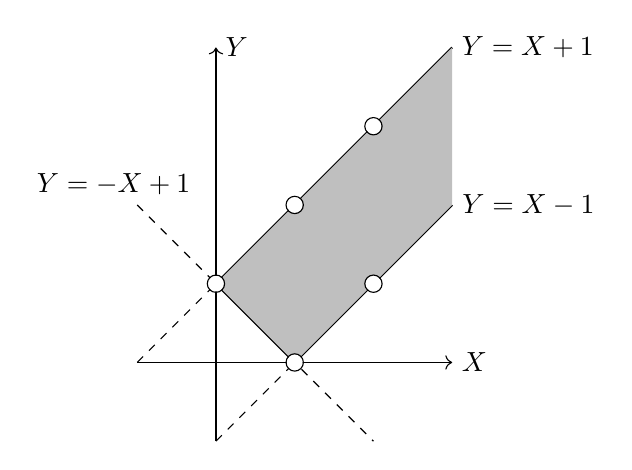
\begin{tikzpicture}[scale=1]
\draw [->] (-1, 0) -- (3, 0) node[right]{$X$}; 
\draw[->] (0, -1) -- (0, 4) node[right]{$Y$}; 
\draw[dashed, domain=-1:2] plot(\x, -\x+1); 
\draw[thick, domain=0:1] plot(\x, -\x+1); 
\draw[dashed, domain=0:3] plot(\x, \x-1); 
\draw[thick, domain=1:2] plot(\x, \x-1); 
\draw[thick, domain=2:3] plot(\x, \x-1) node[right]{$Y=X-1$}; 
\draw[dashed, domain=-1:3] plot(\x, \x+1) node[right]{$Y=X+1$}; 
\draw[thick, domain=0:1] plot(\x, \x+1); 
\draw[thick, domain=1:2] plot(\x, \x+1); 
\draw[thick, domain=2:3] plot(\x, \x+1); 
\fill[lightgray] (1, 0)--(0, 1)--(3, 4)--(3, 2)--cycle;
\fill[fill=white] (0, 1) circle (0.1cm); 
\draw (0, 1) circle (0.11cm); 
\fill[fill=white] (1, 2) circle (0.1cm); 
\draw (1, 2) circle (0.11cm); 
\fill[fill=white] (1, 0) circle (0.1cm); 
\draw (1, 0) circle (0.11cm); 
\fill[fill=white] (2, 1) circle (0.1cm); 
\draw (2, 1) circle (0.11cm); 
\fill[fill=white] (2, 3) circle (0.1cm); 
\draw (2, 3) circle (0.11cm); 
\draw (-1.3, 2) node[above]{$Y=-X+1$}; 
\end{tikzpicture}
\end{center}
\caption{The image $\bP m(\Stab(\bP^1)/\bC)$ in $\bR\bP^2_{\geq 0}$.}
\end{figure}

\begin{comment}
\begin{proof}
\textcolor{red}{maybe we have to change the notation of $\mcA_{p, i, 0}$ (or $\Delta_i$). In this proof, the notation is 
$\mcA_{p, i, 0}=\langle \mcO(i)[p], \mcO(i+1) \rangle$, differs from (6.2)}
Take $\overline{\sigma} \in \mcH_i$. 
%We fix a representative $\sigma=(Z,\mcA_{p,i})$ of the $\bC$-orbit $\overline{\sigma}$.
We have 
\[\bP m(\overline{\sigma})=\left[1: \frac{m_\sigma(\mcO_{\bP^1}(-1))}{m_\sigma(\mcO_x)}:\frac{m_\sigma(\mcO_{\bP^1})}{m_\sigma(\mcO_x)} \right].\]
Put 
\[s:=m_\sigma(\mcO_{\bP^1}(i+1)), t:=m_\sigma(\mcO_{\bP^1}(i)),\]
and
\[X:=\frac{m_\sigma(\mcO_{\bP^1}(-1))}{m_\sigma(\mcO_x)}, Y:=\frac{m_\sigma(\mcO_{\bP^1})}{m_\sigma(\mcO_x)}.\]
We describe $X$ and $Y$ in terms of $s$ and $t$.
By Proposition \ref{prop:P1heart}, we have 
\[ s=|Z(\mcO_{\bP^1}(i+1))|, t=|Z(\mcO_{\bP^1}(i))|.\]
Note that considering the action of $\sqrt{-1}\mathbb{R} \subset \mathbb{C}$, $s$ and $t$ can be arbitrary positive real numbers.
%Considering the action of \textcolor{red}{i=sqrt{-1}} 
%$\sqrt{-1}\bR \subset \bC$ on $\mcH_i$, $s,t$ move in $\mathbb{R}$.

First, we assume that $i=1$. 
\textcolor{red}{seems to be $i=0$?}
By Lemma \ref{lem:generateP1}, we have an exact triangle
\begin{equation}\label{filtration}
\mcO_{\bP^1} \to \mcO_x \to \mcO_{\bP^1}(-1)[1]. 
\end{equation}
If $\mcO_x$ is not $\sigma$-semistable, the exact triangle (\ref{filtration}) is the Harder-Narsimhan filtration of $\mcO_x$ with respect to $\sigma$. If $\mcO_x$ is $\sigma$-semistable, the exact triangle (\ref{filtration}) is the Jordan-H\"older filtration of $\mcO_x$ with respect to $\sigma$. Therefore, we obtain
\begin{align*}
    m_\sigma(\mcO_x) &=  |Z(\mcO_{\bP^1})|+|Z(\mcO_{\bP^1}(-1)[1]| \\
    &=s+t
    %&=m_\sigma(\mcO_{\bP^1})+m_\sigma(\mcO_{\bP^1}(-1)[1])
\end{align*}
and 
\[X=\frac{t}{s+t}, \ Y=\frac{s}{s+t}. \]
So we have 
\[\bP m(\mcH_{-1})=\Delta_{-1}. \]



%\[\bP m(\overline{\sigma})=\left(1: \frac{m_\sigma(\mcO_{\bP^1}(-1))}{m_\sigma(\mcO_{\bP^1}(-1))+m_\sigma(\mcO_{\bP^1})}:\frac{m_\sigma(\mcO_{\bP^1})}{m_\sigma(\mcO_{\bP^1}(-1))+m_\sigma(\mcO_{\bP^1})} \right)\]

\begin{figure}[htb]
\begin{center}
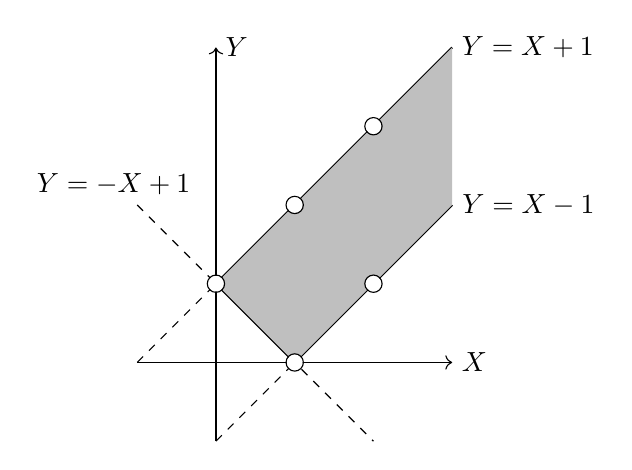
\begin{tikzpicture}[scale=1]
\draw [->] (-1, 0) -- (3, 0) node[right]{$X$}; 
\draw[->] (0, -1) -- (0, 4) node[right]{$Y$}; 
\draw[dashed, domain=-1:2] plot(\x, -\x+1); 
\draw[thick, domain=0:1] plot(\x, -\x+1); 
\draw[dashed, domain=0:3] plot(\x, \x-1); 
\draw[thick, domain=1:2] plot(\x, \x-1); 
\draw[thick, domain=2:3] plot(\x, \x-1) node[right]{$Y=X-1$}; 
\draw[dashed, domain=-1:3] plot(\x, \x+1) node[right]{$Y=X+1$}; 
\draw[thick, domain=0:1] plot(\x, \x+1); 
\draw[thick, domain=1:2] plot(\x, \x+1); 
\draw[thick, domain=2:3] plot(\x, \x+1); 
\fill[lightgray] (1, 0)--(0, 1)--(3, 4)--(3, 2)--cycle;
\fill[fill=white] (0, 1) circle (0.1cm); 
\draw (0, 1) circle (0.11cm); 
\fill[fill=white] (1, 2) circle (0.1cm); 
\draw (1, 2) circle (0.11cm); 
\fill[fill=white] (1, 0) circle (0.1cm); 
\draw (1, 0) circle (0.11cm); 
\fill[fill=white] (2, 1) circle (0.1cm); 
\draw (2, 1) circle (0.11cm); 
\fill[fill=white] (2, 3) circle (0.1cm); 
\draw (2, 3) circle (0.11cm); 
\draw (-1.3, 2) node[above]{$Y=-X+1$}; 
\end{tikzpicture}
\end{center}
\caption{The image $\bP m(\Stab(\bP^1)/\bC)$ in $\bR\bP^2_{\geq 0}$.}
\end{figure}

Next, assume that $i \geq 0$. By Lemma \ref{lem:generateP1}, we have exact triangles
\begin{align*}
 &\mcO_{\bP^1}(k+1)[-1]^{\oplus k+1} \to \mcO_{\bP^1}(-1) \to \mcO_{\bP^1}(k)^{\oplus k-n+1}, \\
    &\mcO_{\bP^1}(k+1)[-1]^{\oplus k} \to \mcO_{\bP^1} \to \mcO_{\bP^1}(k)^{\oplus k-n+1}, \\
    &\mcO_{\bP^1}(i+1) \to \mcO_x \to \mcO_{\bP^1}(i)[1]. 
\end{align*}
\textcolor{red}{what is $k$?}
As in the case of $i=-1$, the above exact triangles are the Harder-Narasimhan or the Jordan-H\"older filtrations with respect to $\sigma$. Therefore, we obtain

\begin{align*}
    m_\sigma(\mcO_x) &=  |Z(\mcO_{\bP^1}(i+1))|+|Z(\mcO_{\bP^1}(i)[1]| \\
    &=s+t,\\
    %&=m_\sigma(\mcO_{\bP^1(i+1)})+m_\sigma(Z(\mcO_{\bP^1}(i)))
    m_\sigma(\mcO_{\bP^1}(-1)) &=  (i+1)|Z(\mcO_{\bP^1}(i+1)[-1])|+(i+2)|Z(\mcO_{\bP^1}(i)| \\
    &=(i+1)s+(i+2)t,\\
   % &=(i+1)m_\sigma(\mcO_{\bP^1(i+1)})+(i+2)m_\sigma((\mcO_{\bP^1}(i)))
    m_\sigma(\mcO_{\bP^1}) &=  i|Z(\mcO_{\bP^1}(i+1))[-1]|+(i+1)|Z(\mcO_{\bP^1}(i)| \\
    &=is+(i+1)t
   % &=im_\sigma(\mcO_{\bP^1(i+1)})+(i+1)m_\sigma((\mcO_{\bP^1}(-1)))
\end{align*}
and 
\[X=\frac{(i+1)s+(k+2)t}{s+t}, \ Y=\frac{is+(i+1)t}{s+t}. \]
Hence, we have 
\[\bP m(\mcH_i)=\Delta_i\]
for $i\geq 0$.

Finally, assume that $i \leq -2$.
As in the case of $i \geq -1$, we obtain
\begin{align*}
    m_\sigma(\mcO_x) &=  |Z(\mcO_{\bP^1}(i+1))|+|Z(\mcO_{\bP^1}(i)[1]| \\
    &=s+t,\\
   % &=m_\sigma(\mcO_{\bP^1(i+1)})+m_\sigma(Z(\mcO_{\bP^1}(i)))
 m_\sigma(\mcO_{\bP^1}(-1)) &=  (-i-1)|Z(\mcO_{\bP^1}(i+1))|+(-i-2)|Z(\mcO_{\bP^1}(i)[1]| \\
 &=(-i-1)s+(-i-2)t,\\
    %&=(-i-1)m_\sigma(\mcO_{\bP^1(i+1)})+(-i-2)m_\sigma((\mcO_{\bP^1}(i)))
m_\sigma(\mcO_{\bP^1}) &=  -i|Z(\mcO_{\bP^1}(i+1))[-1]|+(-i-1)|Z(\mcO_{\bP^1}(i)[1]| \\
&=-is+(-i-1)t
    %&=-im_\sigma(\mcO_{\bP^1(i+1)})+(-i-1)m_\sigma((\mcO_{\bP^1}(-1)))
\end{align*}
and
\[X=\frac{(-i-1)s+(-i-2)t}{s+t}, \ Y=\frac{-is+(-i-1)t}{s+t}. \]
Hence, we have
\[m_\sigma(\mcH_i)=\Delta_i \]
for $i\leq-2$.

\end{proof}
\end{comment}




%=================comment-out================================
\begin{comment}
Using the subset $\Delta\subset\bR\bP^2_{\ge0}$ in \S4.3, 
we define a subset $\Delta^+(\subset\bR\bP^2_{\ge0})$ as follows
\[
\Delta^+:=\Delta\sqcup\{[1:X:Y]\in\bR\bP^2_{\ge0}\mid~Y>-X+1,~Y>X-1,~Y<X+1\}
\]
We clearly have
\[
\Delta\subsetneq\Delta^+\subsetneq\overline{\Delta}. 
\]
Identifying $\bP^{\mcS_3}_{\ge0}$ with $\bR\bP^2_{\ge0}$,
we obtain the followings. 
\begin{thm}
The image $\bP m(\bigsqcup_i \mcH_i)$ is equal to $\Delta^+\backslash\Delta$. 
\end{thm}
\begin{proof}
\end{proof}
\end{comment}

\begin{comment}
%We start with the following easy lemma: 
\begin{lem} \label{lem:generateP1}
For any integer $n \in \bZ$, 
there exist the following exact triangles in $D^b(\bP^1)$: 
\begin{align}
    &\mcO_{\bP^1}^{\oplus n+1} \to \mcO_{\bP^1}(n) \to \mcO_{\bP^1}(-1)[1]^{\oplus n} 
    \quad \mbox{ if } n \geq0, \label{eq:exn>0}\\
    &\mcO_{\bP^1}^{\oplus -n-1} \to \mcO_{\bP^1}(n)[1] \to \mcO_{\bP^1}(-1)[1]^{\oplus -n} 
    \quad \mbox{ if } n \leq -1, \label{eq:exn<0} \\
    &\mcO_{\bP^1} \to \mcO_x \to \mcO_{\bP^1}(-1)[1] \quad \mbox{ for } x \in \bP^1. 
    \label{eq:exOx}
\end{align}
\end{lem}
\begin{proof}
For the readers' convenience, 
we include the first and the third statements here. 
For the first statement, recall that 
we have a semi-orthogonal decomposition 
$D^b(\bP^1)=\langle \mcO_{\bP^1}(-1), \mcO_{\bP^1} \rangle$. 
Hence for each integer $n \geq 0$, 
there exists an exact triangle 
\begin{equation}
    \bigoplus_j \mcO_{\bP^1}[j]^{\oplus k_j} \to \mcO_{\bP^1}(n) \to 
    \bigoplus_j \mcO_{\bP^1}(-1)[j]^{\oplus l_j}. 
\end{equation}
Since $\dR\Hom(\mcO_{\bP^1}, \mcO_{\bP^1}(n))$ (resp, $\dR\Hom(\mcO_{\bP^1}(n), \mcO_{\bP^1}(-1))$) 
is concentrated in degree $0$ (resp. $1$), 
\end{proof}
\end{comment}

\begin{comment}
\begin{thm}
The image ${\bP m}(\bigsqcup_i \mcH_i) \subset \bP^\mcS_{\geq 0}$ is contained in the boundary of the closure 
$\overline{{\bP m}(\Geo(\bP^1)/\bC)} \cong \overline{D}$. 
More precisely, we have the commutative diagram: 
\[
\xymatrix{
&\overline{{\bP m}(\Geo(\bP^1)/\bC)} \ar[r]^-\sim 
&\overline{D} \\
&{\bP m}(\bigsqcup_i \mcH_i) \ar@{_{(}->}[u] \ar[r]^-\sim 
&\partial D \setminus \bZ. \ar@{_{(}->}[u]. 
}
\]
\end{thm}
\begin{proof}
By Lemmas \ref{lem:generateP1} and \ref{lem:degenstable}, 
the image of degenerated stability conditions under the map $m$ 
is determined by the coordinates at $\mcO_{\bP^1}(-1), \mcO_{\bP^1}$, 
and $\mcO_x$ for $x \in \bP^1$. 
\end{proof}
\end{comment}

%============================================================
\bibliographystyle{alpha}
\bibliography{maths}


\end{document}
